\chapter{Steiner Forest algorithms}

\section{Problem description}
Steiner Forest Problem (SFP)\\
Given an undirected graph $G = (V, E)$, a cost function on edges $c : E \rightarrow Q^+$, and a collection of disjoint subsets of $V$, $S_1, \dots S_k$, find a minimum cost subgraph in which each pair of vertices belonging to the same set $S_i$ is connected.
For $k = 1$ the problem is known as Steiner Tree Problem (STP).

\section{Primal-Dual Method algorithm}
Local searches written in our framework were compared to a 2-approximation algorithm described by Vazirani [Vazirani]. As far as we know, it's the best approximation algorithm for a SFP known to date.

\section{Create and break cycle local search}
Given some solution to Steiner Forest Problem ,,Create and break cycle'' (CBC) local search changes it by randomly adding edge between solution's vertices. If added edge created a cycle then the heaviest edge from this cycle is removed. It's obvious that obtained graph is still a feasible solution. After described operation it might happen that some edges are no longer needed like for example edges adjacent to leafs that don't belong to $S_i$ for any $i \in \{1, \dots k\}$. Therefore pruning procedure is used to ensure that only essential edges remains which might lead to further fitness improvement.

\section{Minimum spanning tree of active vertices local search}
,,MST of active vertices'' (MSTAV) local search starts with some feasible solution of SFP. At each step a new solution is created by computing a pruned minimum spanning tree of $G'$ which is a subgraph of $G$ induced by some set of vertices $V'$ called active vertices. $V'$ is obtained from vertices belonging to the previous solution after randomly applying one of the following operations:
\begin{itemize}
\item add a random vertex that's not already in the set,
\item remove a random vertex from the set,
\item do both operations described above.
\end{itemize}

Note that it might happen that there is no feasible solution in $G'$. Therefore at the end of each step local search checks whether proposed solution is feasible and if it is not then it reverts any changes.

\section{Benchmarks}
To compare the algorithms we have used our randomly generated tests and a subset of SteinLib\footnote{\url{steinlib.zib.de}} tests for Steiner Tree Problem.
TODO: opisac kodowanie nazwy testow

\section{Results}
WIP

\subsection{Comparison of hill climbing and simulated annealing convergence}
STUB text\\
TODO: krotko napisac, ze SA dziala w CBC, ale nie w MSTAV i dlaczego\\
dalej bede rozwazal CBC HillClimb + CBC SA 1e-5\\
\pgfsetplotmarksize{0pt}
\begin{figure}
 \centering
 \caption{\label{CBC-01dEV100K30}CBC-01dEV100K30},
 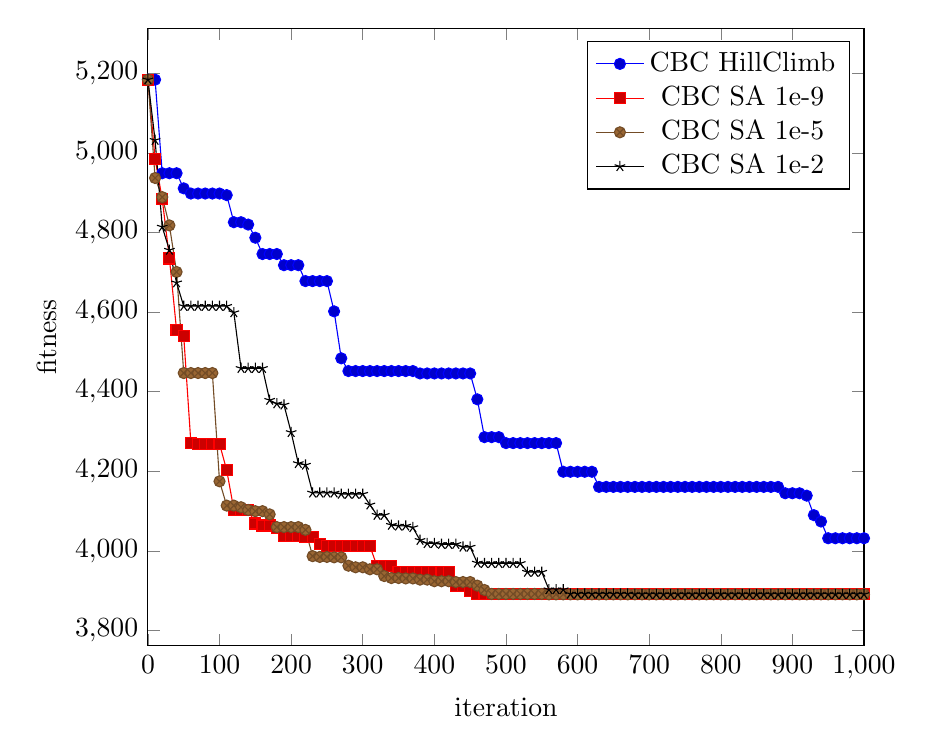
\begin{tikzpicture}
 \begin{axis}[
   width=0.75\textwidth,
   scale only axis,
   xlabel=iteration,
   ylabel=fitness,
   xmin=0,xmax=1000,
   domain=0:1000]
   \addplot coordinates {
     (0,5184)
     (10,5184)
     (20,4949)
     (30,4949)
     (40,4949)
     (50,4911)
     (60,4898)
     (70,4898)
     (80,4898)
     (90,4898)
     (100,4898)
     (110,4894)
     (120,4826)
     (130,4826)
     (140,4820)
     (150,4787)
     (160,4746)
     (170,4746)
     (180,4746)
     (190,4718)
     (200,4718)
     (210,4718)
     (220,4678)
     (230,4678)
     (240,4678)
     (250,4678)
     (260,4602)
     (270,4484)
     (280,4452)
     (290,4452)
     (300,4452)
     (310,4452)
     (320,4452)
     (330,4452)
     (340,4452)
     (350,4452)
     (360,4452)
     (370,4452)
     (380,4446)
     (390,4446)
     (400,4446)
     (410,4446)
     (420,4446)
     (430,4446)
     (440,4446)
     (450,4446)
     (460,4381)
     (470,4286)
     (480,4286)
     (490,4286)
     (500,4271)
     (510,4271)
     (520,4271)
     (530,4271)
     (540,4271)
     (550,4271)
     (560,4271)
     (570,4271)
     (580,4199)
     (590,4199)
     (600,4199)
     (610,4199)
     (620,4199)
     (630,4161)
     (640,4161)
     (650,4161)
     (660,4161)
     (670,4161)
     (680,4161)
     (690,4161)
     (700,4161)
     (710,4161)
     (720,4161)
     (730,4161)
     (740,4161)
     (750,4161)
     (760,4161)
     (770,4161)
     (780,4161)
     (790,4161)
     (800,4161)
     (810,4161)
     (820,4161)
     (830,4161)
     (840,4161)
     (850,4161)
     (860,4161)
     (870,4161)
     (880,4161)
     (890,4145)
     (900,4145)
     (910,4145)
     (920,4139)
     (930,4090)
     (940,4074)
     (950,4032)
     (960,4032)
     (970,4032)
     (980,4032)
     (990,4032)
     (1000,4032)
   };
   \addlegendentry{CBC HillClimb}
   \addplot coordinates {
     (0,5184)
     (10,4985)
     (20,4884)
     (30,4735)
     (40,4555)
     (50,4540)
     (60,4271)
     (70,4269)
     (80,4269)
     (90,4269)
     (100,4269)
     (110,4203)
     (120,4104)
     (130,4103)
     (140,4103)
     (150,4069)
     (160,4064)
     (170,4064)
     (180,4057)
     (190,4038)
     (200,4038)
     (210,4038)
     (220,4036)
     (230,4036)
     (240,4018)
     (250,4013)
     (260,4013)
     (270,4013)
     (280,4012)
     (290,4012)
     (300,4012)
     (310,4012)
     (320,3962)
     (330,3962)
     (340,3962)
     (350,3948)
     (360,3948)
     (370,3948)
     (380,3948)
     (390,3948)
     (400,3948)
     (410,3948)
     (420,3948)
     (430,3911)
     (440,3911)
     (450,3900)
     (460,3891)
     (470,3891)
     (480,3891)
     (490,3891)
     (500,3891)
     (510,3891)
     (520,3891)
     (530,3891)
     (540,3891)
     (550,3891)
     (560,3891)
     (570,3891)
     (580,3891)
     (590,3891)
     (600,3891)
     (610,3891)
     (620,3891)
     (630,3891)
     (640,3891)
     (650,3891)
     (660,3891)
     (670,3891)
     (680,3891)
     (690,3891)
     (700,3891)
     (710,3891)
     (720,3891)
     (730,3891)
     (740,3891)
     (750,3891)
     (760,3891)
     (770,3891)
     (780,3891)
     (790,3891)
     (800,3891)
     (810,3891)
     (820,3891)
     (830,3891)
     (840,3891)
     (850,3891)
     (860,3891)
     (870,3891)
     (880,3891)
     (890,3891)
     (900,3891)
     (910,3891)
     (920,3891)
     (930,3891)
     (940,3891)
     (950,3891)
     (960,3891)
     (970,3891)
     (980,3891)
     (990,3891)
     (1000,3891)
   };
   \addlegendentry{CBC SA 1e-9}
   \addplot coordinates {
     (0,5184)
     (10,4937)
     (20,4889)
     (30,4818)
     (40,4701)
     (50,4447)
     (60,4447)
     (70,4447)
     (80,4447)
     (90,4447)
     (100,4175)
     (110,4114)
     (120,4114)
     (130,4110)
     (140,4103)
     (150,4100)
     (160,4100)
     (170,4092)
     (180,4060)
     (190,4060)
     (200,4060)
     (210,4060)
     (220,4053)
     (230,3987)
     (240,3985)
     (250,3985)
     (260,3984)
     (270,3984)
     (280,3963)
     (290,3959)
     (300,3959)
     (310,3954)
     (320,3954)
     (330,3937)
     (340,3932)
     (350,3932)
     (360,3931)
     (370,3931)
     (380,3928)
     (390,3928)
     (400,3924)
     (410,3924)
     (420,3924)
     (430,3922)
     (440,3922)
     (450,3922)
     (460,3913)
     (470,3902)
     (480,3892)
     (490,3892)
     (500,3892)
     (510,3892)
     (520,3892)
     (530,3892)
     (540,3892)
     (550,3892)
     (560,3891)
     (570,3891)
     (580,3891)
     (590,3891)
     (600,3891)
     (610,3891)
     (620,3891)
     (630,3891)
     (640,3891)
     (650,3891)
     (660,3891)
     (670,3891)
     (680,3891)
     (690,3891)
     (700,3891)
     (710,3891)
     (720,3891)
     (730,3891)
     (740,3891)
     (750,3891)
     (760,3891)
     (770,3891)
     (780,3891)
     (790,3891)
     (800,3891)
     (810,3891)
     (820,3891)
     (830,3891)
     (840,3891)
     (850,3891)
     (860,3891)
     (870,3891)
     (880,3891)
     (890,3891)
     (900,3891)
     (910,3891)
     (920,3891)
     (930,3891)
     (940,3891)
     (950,3891)
     (960,3891)
     (970,3891)
     (980,3891)
     (990,3891)
     (1000,3891)
   };
   \addlegendentry{CBC SA 1e-5}
   \addplot coordinates {
     (0,5184)
     (10,5032)
     (20,4814)
     (30,4756)
     (40,4674)
     (50,4615)
     (60,4615)
     (70,4615)
     (80,4615)
     (90,4615)
     (100,4615)
     (110,4615)
     (120,4599)
     (130,4459)
     (140,4459)
     (150,4459)
     (160,4459)
     (170,4379)
     (180,4370)
     (190,4367)
     (200,4298)
     (210,4220)
     (220,4216)
     (230,4146)
     (240,4146)
     (250,4146)
     (260,4146)
     (270,4143)
     (280,4143)
     (290,4143)
     (300,4143)
     (310,4116)
     (320,4090)
     (330,4090)
     (340,4065)
     (350,4063)
     (360,4063)
     (370,4059)
     (380,4027)
     (390,4019)
     (400,4019)
     (410,4017)
     (420,4017)
     (430,4017)
     (440,4010)
     (450,4010)
     (460,3970)
     (470,3969)
     (480,3969)
     (490,3969)
     (500,3969)
     (510,3969)
     (520,3969)
     (530,3947)
     (540,3947)
     (550,3947)
     (560,3903)
     (570,3903)
     (580,3903)
     (590,3892)
     (600,3892)
     (610,3892)
     (620,3892)
     (630,3892)
     (640,3892)
     (650,3892)
     (660,3892)
     (670,3892)
     (680,3891)
     (690,3891)
     (700,3891)
     (710,3891)
     (720,3891)
     (730,3891)
     (740,3891)
     (750,3891)
     (760,3891)
     (770,3891)
     (780,3891)
     (790,3891)
     (800,3891)
     (810,3891)
     (820,3891)
     (830,3891)
     (840,3891)
     (850,3891)
     (860,3891)
     (870,3891)
     (880,3891)
     (890,3891)
     (900,3891)
     (910,3891)
     (920,3891)
     (930,3891)
     (940,3891)
     (950,3891)
     (960,3891)
     (970,3891)
     (980,3891)
     (990,3891)
     (1000,3891)
   };
   \addlegendentry{CBC SA 1e-2}
 \end{axis}
 \end{tikzpicture}
\end{figure}

\pgfsetplotmarksize{0pt}
 \centering
 \caption{\label{CBC-02dEV100K30}CBC-02dEV100K30},
 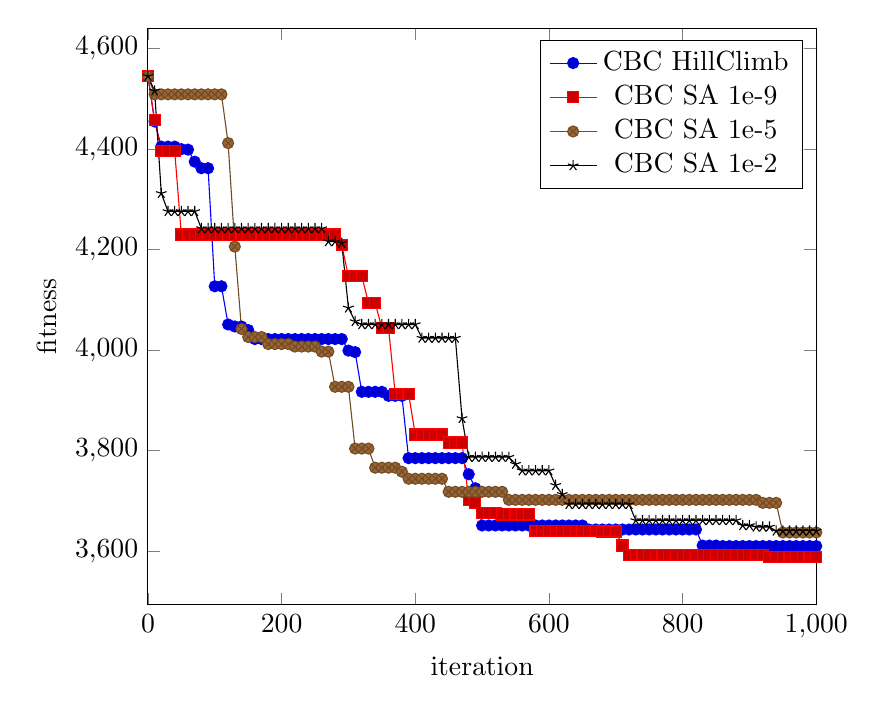
\begin{tikzpicture}
 \begin{axis}[
   width=0.7\textwidth,
   scale only axis,
   xlabel=iteration,
   ylabel=fitness,
   xmin=0,xmax=1000,
   domain=0:1000]
   \addplot coordinates {
     (0,4545)
     (10,4455)
     (20,4405)
     (30,4405)
     (40,4405)
     (50,4400)
     (60,4399)
     (70,4375)
     (80,4362)
     (90,4362)
     (100,4127)
     (110,4127)
     (120,4051)
     (130,4047)
     (140,4047)
     (150,4040)
     (160,4022)
     (170,4022)
     (180,4022)
     (190,4022)
     (200,4022)
     (210,4022)
     (220,4022)
     (230,4022)
     (240,4022)
     (250,4022)
     (260,4022)
     (270,4022)
     (280,4022)
     (290,4022)
     (300,3999)
     (310,3996)
     (320,3917)
     (330,3917)
     (340,3917)
     (350,3917)
     (360,3909)
     (370,3909)
     (380,3909)
     (390,3785)
     (400,3785)
     (410,3785)
     (420,3785)
     (430,3785)
     (440,3785)
     (450,3785)
     (460,3785)
     (470,3785)
     (480,3753)
     (490,3725)
     (500,3651)
     (510,3651)
     (520,3651)
     (530,3651)
     (540,3651)
     (550,3651)
     (560,3651)
     (570,3651)
     (580,3651)
     (590,3651)
     (600,3651)
     (610,3651)
     (620,3651)
     (630,3651)
     (640,3651)
     (650,3651)
     (660,3643)
     (670,3643)
     (680,3643)
     (690,3643)
     (700,3643)
     (710,3643)
     (720,3643)
     (730,3643)
     (740,3643)
     (750,3643)
     (760,3643)
     (770,3643)
     (780,3643)
     (790,3643)
     (800,3643)
     (810,3643)
     (820,3643)
     (830,3611)
     (840,3611)
     (850,3611)
     (860,3610)
     (870,3610)
     (880,3610)
     (890,3610)
     (900,3610)
     (910,3610)
     (920,3610)
     (930,3610)
     (940,3610)
     (950,3610)
     (960,3610)
     (970,3610)
     (980,3610)
     (990,3610)
     (1000,3610)
   };
   \addlegendentry{CBC HillClimb}
   \addplot coordinates {
     (0,4545)
     (10,4458)
     (20,4397)
     (30,4397)
     (40,4397)
     (50,4230)
     (60,4230)
     (70,4230)
     (80,4230)
     (90,4230)
     (100,4230)
     (110,4230)
     (120,4230)
     (130,4230)
     (140,4230)
     (150,4230)
     (160,4230)
     (170,4230)
     (180,4230)
     (190,4230)
     (200,4230)
     (210,4230)
     (220,4230)
     (230,4230)
     (240,4230)
     (250,4230)
     (260,4230)
     (270,4230)
     (280,4230)
     (290,4209)
     (300,4147)
     (310,4147)
     (320,4147)
     (330,4094)
     (340,4094)
     (350,4044)
     (360,4044)
     (370,3913)
     (380,3913)
     (390,3913)
     (400,3832)
     (410,3832)
     (420,3832)
     (430,3832)
     (440,3832)
     (450,3816)
     (460,3816)
     (470,3816)
     (480,3701)
     (490,3696)
     (500,3676)
     (510,3676)
     (520,3676)
     (530,3673)
     (540,3673)
     (550,3673)
     (560,3673)
     (570,3673)
     (580,3640)
     (590,3640)
     (600,3640)
     (610,3640)
     (620,3640)
     (630,3640)
     (640,3640)
     (650,3640)
     (660,3640)
     (670,3640)
     (680,3639)
     (690,3639)
     (700,3639)
     (710,3611)
     (720,3593)
     (730,3593)
     (740,3593)
     (750,3593)
     (760,3593)
     (770,3593)
     (780,3593)
     (790,3593)
     (800,3593)
     (810,3593)
     (820,3593)
     (830,3593)
     (840,3593)
     (850,3593)
     (860,3593)
     (870,3593)
     (880,3593)
     (890,3593)
     (900,3593)
     (910,3593)
     (920,3593)
     (930,3589)
     (940,3589)
     (950,3589)
     (960,3589)
     (970,3589)
     (980,3589)
     (990,3589)
     (1000,3589)
   };
   \addlegendentry{CBC SA 1e-9}
   \addplot coordinates {
     (0,4545)
     (10,4509)
     (20,4509)
     (30,4509)
     (40,4509)
     (50,4509)
     (60,4509)
     (70,4509)
     (80,4509)
     (90,4509)
     (100,4509)
     (110,4509)
     (120,4412)
     (130,4206)
     (140,4042)
     (150,4026)
     (160,4026)
     (170,4026)
     (180,4012)
     (190,4012)
     (200,4012)
     (210,4012)
     (220,4007)
     (230,4007)
     (240,4007)
     (250,4007)
     (260,3997)
     (270,3997)
     (280,3927)
     (290,3927)
     (300,3927)
     (310,3804)
     (320,3804)
     (330,3804)
     (340,3766)
     (350,3766)
     (360,3766)
     (370,3766)
     (380,3758)
     (390,3744)
     (400,3744)
     (410,3744)
     (420,3744)
     (430,3744)
     (440,3744)
     (450,3718)
     (460,3718)
     (470,3718)
     (480,3718)
     (490,3718)
     (500,3718)
     (510,3718)
     (520,3718)
     (530,3718)
     (540,3702)
     (550,3702)
     (560,3702)
     (570,3702)
     (580,3702)
     (590,3702)
     (600,3702)
     (610,3702)
     (620,3702)
     (630,3702)
     (640,3702)
     (650,3702)
     (660,3702)
     (670,3702)
     (680,3702)
     (690,3702)
     (700,3702)
     (710,3702)
     (720,3702)
     (730,3702)
     (740,3702)
     (750,3702)
     (760,3702)
     (770,3702)
     (780,3702)
     (790,3702)
     (800,3702)
     (810,3702)
     (820,3702)
     (830,3702)
     (840,3702)
     (850,3702)
     (860,3702)
     (870,3702)
     (880,3702)
     (890,3702)
     (900,3702)
     (910,3702)
     (920,3696)
     (930,3696)
     (940,3696)
     (950,3637)
     (960,3637)
     (970,3637)
     (980,3637)
     (990,3637)
     (1000,3637)
   };
   \addlegendentry{CBC SA 1e-5}
   \addplot coordinates {
     (0,4545)
     (10,4516)
     (20,4312)
     (30,4276)
     (40,4276)
     (50,4276)
     (60,4276)
     (70,4276)
     (80,4242)
     (90,4242)
     (100,4242)
     (110,4242)
     (120,4242)
     (130,4242)
     (140,4242)
     (150,4242)
     (160,4242)
     (170,4242)
     (180,4242)
     (190,4242)
     (200,4242)
     (210,4242)
     (220,4242)
     (230,4242)
     (240,4242)
     (250,4242)
     (260,4242)
     (270,4216)
     (280,4216)
     (290,4213)
     (300,4084)
     (310,4057)
     (320,4051)
     (330,4051)
     (340,4051)
     (350,4051)
     (360,4051)
     (370,4051)
     (380,4051)
     (390,4051)
     (400,4051)
     (410,4024)
     (420,4024)
     (430,4024)
     (440,4024)
     (450,4024)
     (460,4024)
     (470,3864)
     (480,3787)
     (490,3787)
     (500,3787)
     (510,3787)
     (520,3787)
     (530,3787)
     (540,3787)
     (550,3773)
     (560,3760)
     (570,3760)
     (580,3760)
     (590,3760)
     (600,3760)
     (610,3731)
     (620,3713)
     (630,3693)
     (640,3693)
     (650,3693)
     (660,3693)
     (670,3693)
     (680,3693)
     (690,3693)
     (700,3693)
     (710,3693)
     (720,3693)
     (730,3661)
     (740,3661)
     (750,3661)
     (760,3661)
     (770,3661)
     (780,3661)
     (790,3661)
     (800,3661)
     (810,3661)
     (820,3661)
     (830,3661)
     (840,3661)
     (850,3661)
     (860,3661)
     (870,3661)
     (880,3661)
     (890,3651)
     (900,3651)
     (910,3648)
     (920,3648)
     (930,3648)
     (940,3640)
     (950,3640)
     (960,3640)
     (970,3640)
     (980,3640)
     (990,3640)
     (1000,3640)
   };
   \addlegendentry{CBC SA 1e-2}
 \end{axis}
 \end{tikzpicture}

\pgfsetplotmarksize{0pt}
 \centering
 \caption{\label{CBC-alue2087}CBC-alue2087},
 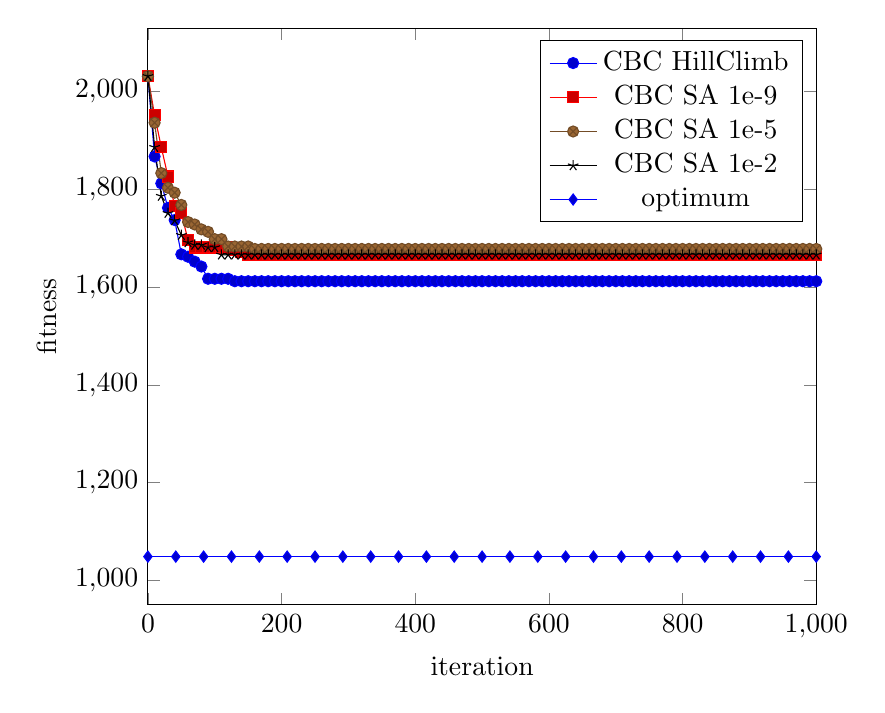
\begin{tikzpicture}
 \begin{axis}[
   width=0.7\textwidth,
   scale only axis,
   xlabel=iteration,
   ylabel=fitness,
   xmin=0,xmax=1000,
   domain=0:1000]
   \addplot coordinates {
     (0,2031)
     (10,1867)
     (20,1812)
     (30,1762)
     (40,1737)
     (50,1667)
     (60,1662)
     (70,1652)
     (80,1642)
     (90,1617)
     (100,1617)
     (110,1617)
     (120,1617)
     (130,1612)
     (140,1612)
     (150,1612)
     (160,1612)
     (170,1612)
     (180,1612)
     (190,1612)
     (200,1612)
     (210,1612)
     (220,1612)
     (230,1612)
     (240,1612)
     (250,1612)
     (260,1612)
     (270,1612)
     (280,1612)
     (290,1612)
     (300,1612)
     (310,1612)
     (320,1612)
     (330,1612)
     (340,1612)
     (350,1612)
     (360,1612)
     (370,1612)
     (380,1612)
     (390,1612)
     (400,1612)
     (410,1612)
     (420,1612)
     (430,1612)
     (440,1612)
     (450,1612)
     (460,1612)
     (470,1612)
     (480,1612)
     (490,1612)
     (500,1612)
     (510,1612)
     (520,1612)
     (530,1612)
     (540,1612)
     (550,1612)
     (560,1612)
     (570,1612)
     (580,1612)
     (590,1612)
     (600,1612)
     (610,1612)
     (620,1612)
     (630,1612)
     (640,1612)
     (650,1612)
     (660,1612)
     (670,1612)
     (680,1612)
     (690,1612)
     (700,1612)
     (710,1612)
     (720,1612)
     (730,1612)
     (740,1612)
     (750,1612)
     (760,1612)
     (770,1612)
     (780,1612)
     (790,1612)
     (800,1612)
     (810,1612)
     (820,1612)
     (830,1612)
     (840,1612)
     (850,1612)
     (860,1612)
     (870,1612)
     (880,1612)
     (890,1612)
     (900,1612)
     (910,1612)
     (920,1612)
     (930,1612)
     (940,1612)
     (950,1612)
     (960,1612)
     (970,1612)
     (980,1612)
     (990,1612)
     (1000,1612)
   };
   \addlegendentry{CBC HillClimb}
   \addplot coordinates {
     (0,2031)
     (10,1951)
     (20,1886)
     (30,1826)
     (40,1766)
     (50,1751)
     (60,1696)
     (70,1681)
     (80,1681)
     (90,1681)
     (100,1681)
     (110,1681)
     (120,1681)
     (130,1676)
     (140,1671)
     (150,1666)
     (160,1666)
     (170,1666)
     (180,1666)
     (190,1666)
     (200,1666)
     (210,1666)
     (220,1666)
     (230,1666)
     (240,1666)
     (250,1666)
     (260,1666)
     (270,1666)
     (280,1666)
     (290,1666)
     (300,1666)
     (310,1666)
     (320,1666)
     (330,1666)
     (340,1666)
     (350,1666)
     (360,1666)
     (370,1666)
     (380,1666)
     (390,1666)
     (400,1666)
     (410,1666)
     (420,1666)
     (430,1666)
     (440,1666)
     (450,1666)
     (460,1666)
     (470,1666)
     (480,1666)
     (490,1666)
     (500,1666)
     (510,1666)
     (520,1666)
     (530,1666)
     (540,1666)
     (550,1666)
     (560,1666)
     (570,1666)
     (580,1666)
     (590,1666)
     (600,1666)
     (610,1666)
     (620,1666)
     (630,1666)
     (640,1666)
     (650,1666)
     (660,1666)
     (670,1666)
     (680,1666)
     (690,1666)
     (700,1666)
     (710,1666)
     (720,1666)
     (730,1666)
     (740,1666)
     (750,1666)
     (760,1666)
     (770,1666)
     (780,1666)
     (790,1666)
     (800,1666)
     (810,1666)
     (820,1666)
     (830,1666)
     (840,1666)
     (850,1666)
     (860,1666)
     (870,1666)
     (880,1666)
     (890,1666)
     (900,1666)
     (910,1666)
     (920,1666)
     (930,1666)
     (940,1666)
     (950,1666)
     (960,1666)
     (970,1666)
     (980,1666)
     (990,1666)
     (1000,1666)
   };
   \addlegendentry{CBC SA 1e-9}
   \addplot coordinates {
     (0,2031)
     (10,1936)
     (20,1833)
     (30,1803)
     (40,1793)
     (50,1768)
     (60,1733)
     (70,1728)
     (80,1718)
     (90,1713)
     (100,1698)
     (110,1698)
     (120,1683)
     (130,1683)
     (140,1683)
     (150,1683)
     (160,1678)
     (170,1678)
     (180,1678)
     (190,1678)
     (200,1678)
     (210,1678)
     (220,1678)
     (230,1678)
     (240,1678)
     (250,1678)
     (260,1678)
     (270,1678)
     (280,1678)
     (290,1678)
     (300,1678)
     (310,1678)
     (320,1678)
     (330,1678)
     (340,1678)
     (350,1678)
     (360,1678)
     (370,1678)
     (380,1678)
     (390,1678)
     (400,1678)
     (410,1678)
     (420,1678)
     (430,1678)
     (440,1678)
     (450,1678)
     (460,1678)
     (470,1678)
     (480,1678)
     (490,1678)
     (500,1678)
     (510,1678)
     (520,1678)
     (530,1678)
     (540,1678)
     (550,1678)
     (560,1678)
     (570,1678)
     (580,1678)
     (590,1678)
     (600,1678)
     (610,1678)
     (620,1678)
     (630,1678)
     (640,1678)
     (650,1678)
     (660,1678)
     (670,1678)
     (680,1678)
     (690,1678)
     (700,1678)
     (710,1678)
     (720,1678)
     (730,1678)
     (740,1678)
     (750,1678)
     (760,1678)
     (770,1678)
     (780,1678)
     (790,1678)
     (800,1678)
     (810,1678)
     (820,1678)
     (830,1678)
     (840,1678)
     (850,1678)
     (860,1678)
     (870,1678)
     (880,1678)
     (890,1678)
     (900,1678)
     (910,1678)
     (920,1678)
     (930,1678)
     (940,1678)
     (950,1678)
     (960,1678)
     (970,1678)
     (980,1678)
     (990,1678)
     (1000,1678)
   };
   \addlegendentry{CBC SA 1e-5}
   \addplot coordinates {
     (0,2031)
     (10,1886)
     (20,1786)
     (30,1751)
     (40,1736)
     (50,1706)
     (60,1691)
     (70,1686)
     (80,1686)
     (90,1681)
     (100,1681)
     (110,1666)
     (120,1666)
     (130,1666)
     (140,1666)
     (150,1666)
     (160,1666)
     (170,1666)
     (180,1666)
     (190,1666)
     (200,1666)
     (210,1666)
     (220,1666)
     (230,1666)
     (240,1666)
     (250,1666)
     (260,1666)
     (270,1666)
     (280,1666)
     (290,1666)
     (300,1666)
     (310,1666)
     (320,1666)
     (330,1666)
     (340,1666)
     (350,1666)
     (360,1666)
     (370,1666)
     (380,1666)
     (390,1666)
     (400,1666)
     (410,1666)
     (420,1666)
     (430,1666)
     (440,1666)
     (450,1666)
     (460,1666)
     (470,1666)
     (480,1666)
     (490,1666)
     (500,1666)
     (510,1666)
     (520,1666)
     (530,1666)
     (540,1666)
     (550,1666)
     (560,1666)
     (570,1666)
     (580,1666)
     (590,1666)
     (600,1666)
     (610,1666)
     (620,1666)
     (630,1666)
     (640,1666)
     (650,1666)
     (660,1666)
     (670,1666)
     (680,1666)
     (690,1666)
     (700,1666)
     (710,1666)
     (720,1666)
     (730,1666)
     (740,1666)
     (750,1666)
     (760,1666)
     (770,1666)
     (780,1666)
     (790,1666)
     (800,1666)
     (810,1666)
     (820,1666)
     (830,1666)
     (840,1666)
     (850,1666)
     (860,1666)
     (870,1666)
     (880,1666)
     (890,1666)
     (900,1666)
     (910,1666)
     (920,1666)
     (930,1666)
     (940,1666)
     (950,1666)
     (960,1666)
     (970,1666)
     (980,1666)
     (990,1666)
     (1000,1666)
   };
   \addlegendentry{CBC SA 1e-2}
   \addplot {1049.000000};
   \addlegendentry{optimum}
 \end{axis}
 \end{tikzpicture}

\pgfsetplotmarksize{0pt}
 \centering
 \caption{\label{CBC-berlin52}CBC-berlin52},
 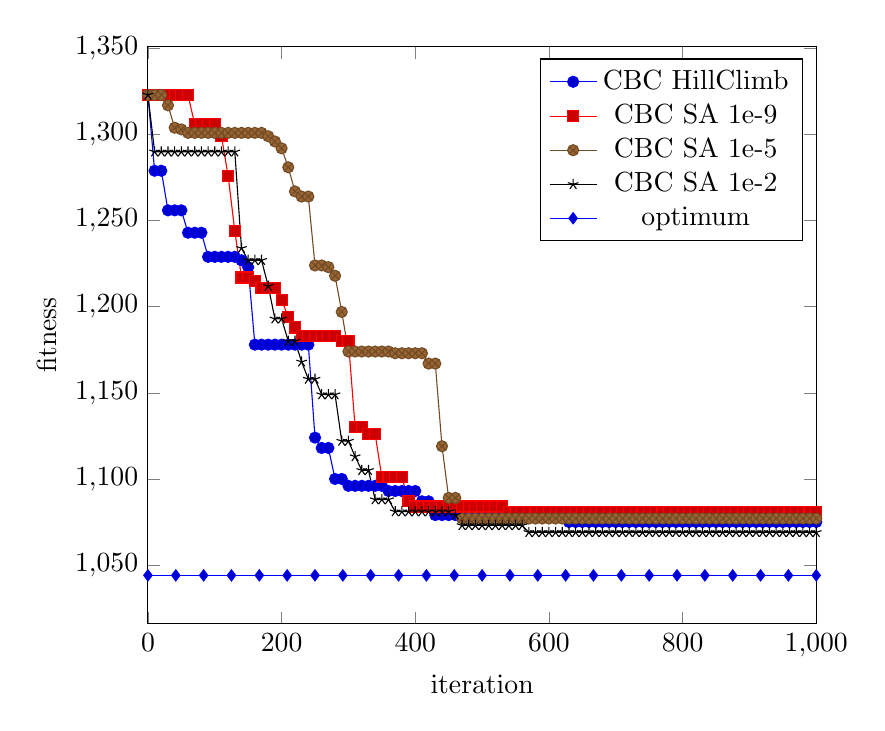
\begin{tikzpicture}
 \begin{axis}[
   width=0.7\textwidth,
   scale only axis,
   xlabel=iteration,
   ylabel=fitness,
   xmin=0,xmax=1000,
   domain=0:1000]
   \addplot coordinates {
     (0,1323)
     (10,1279)
     (20,1279)
     (30,1256)
     (40,1256)
     (50,1256)
     (60,1243)
     (70,1243)
     (80,1243)
     (90,1229)
     (100,1229)
     (110,1229)
     (120,1229)
     (130,1229)
     (140,1227)
     (150,1223)
     (160,1178)
     (170,1178)
     (180,1178)
     (190,1178)
     (200,1178)
     (210,1178)
     (220,1178)
     (230,1178)
     (240,1178)
     (250,1124)
     (260,1118)
     (270,1118)
     (280,1100)
     (290,1100)
     (300,1096)
     (310,1096)
     (320,1096)
     (330,1096)
     (340,1096)
     (350,1096)
     (360,1093)
     (370,1093)
     (380,1093)
     (390,1093)
     (400,1093)
     (410,1087)
     (420,1087)
     (430,1079)
     (440,1079)
     (450,1079)
     (460,1079)
     (470,1079)
     (480,1078)
     (490,1078)
     (500,1078)
     (510,1078)
     (520,1078)
     (530,1078)
     (540,1078)
     (550,1078)
     (560,1078)
     (570,1078)
     (580,1078)
     (590,1078)
     (600,1078)
     (610,1078)
     (620,1078)
     (630,1075)
     (640,1075)
     (650,1075)
     (660,1075)
     (670,1075)
     (680,1075)
     (690,1075)
     (700,1075)
     (710,1075)
     (720,1075)
     (730,1075)
     (740,1075)
     (750,1075)
     (760,1075)
     (770,1075)
     (780,1075)
     (790,1075)
     (800,1075)
     (810,1075)
     (820,1075)
     (830,1075)
     (840,1075)
     (850,1075)
     (860,1075)
     (870,1075)
     (880,1075)
     (890,1075)
     (900,1075)
     (910,1075)
     (920,1075)
     (930,1075)
     (940,1075)
     (950,1075)
     (960,1075)
     (970,1075)
     (980,1075)
     (990,1075)
     (1000,1075)
   };
   \addlegendentry{CBC HillClimb}
   \addplot coordinates {
     (0,1323)
     (10,1323)
     (20,1323)
     (30,1323)
     (40,1323)
     (50,1323)
     (60,1323)
     (70,1306)
     (80,1306)
     (90,1306)
     (100,1306)
     (110,1299)
     (120,1276)
     (130,1244)
     (140,1217)
     (150,1217)
     (160,1215)
     (170,1211)
     (180,1211)
     (190,1211)
     (200,1204)
     (210,1194)
     (220,1188)
     (230,1183)
     (240,1183)
     (250,1183)
     (260,1183)
     (270,1183)
     (280,1183)
     (290,1180)
     (300,1180)
     (310,1130)
     (320,1130)
     (330,1126)
     (340,1126)
     (350,1101)
     (360,1101)
     (370,1101)
     (380,1101)
     (390,1087)
     (400,1084)
     (410,1084)
     (420,1084)
     (430,1084)
     (440,1084)
     (450,1084)
     (460,1084)
     (470,1084)
     (480,1084)
     (490,1084)
     (500,1084)
     (510,1084)
     (520,1084)
     (530,1084)
     (540,1081)
     (550,1081)
     (560,1081)
     (570,1081)
     (580,1081)
     (590,1081)
     (600,1081)
     (610,1081)
     (620,1081)
     (630,1081)
     (640,1081)
     (650,1081)
     (660,1081)
     (670,1081)
     (680,1081)
     (690,1081)
     (700,1081)
     (710,1081)
     (720,1081)
     (730,1081)
     (740,1081)
     (750,1081)
     (760,1081)
     (770,1081)
     (780,1081)
     (790,1081)
     (800,1081)
     (810,1081)
     (820,1081)
     (830,1081)
     (840,1081)
     (850,1081)
     (860,1081)
     (870,1081)
     (880,1081)
     (890,1081)
     (900,1081)
     (910,1081)
     (920,1081)
     (930,1081)
     (940,1081)
     (950,1081)
     (960,1081)
     (970,1081)
     (980,1081)
     (990,1081)
     (1000,1081)
   };
   \addlegendentry{CBC SA 1e-9}
   \addplot coordinates {
     (0,1323)
     (10,1323)
     (20,1323)
     (30,1317)
     (40,1304)
     (50,1303)
     (60,1301)
     (70,1301)
     (80,1301)
     (90,1301)
     (100,1301)
     (110,1301)
     (120,1301)
     (130,1301)
     (140,1301)
     (150,1301)
     (160,1301)
     (170,1301)
     (180,1299)
     (190,1296)
     (200,1292)
     (210,1281)
     (220,1267)
     (230,1264)
     (240,1264)
     (250,1224)
     (260,1224)
     (270,1223)
     (280,1218)
     (290,1197)
     (300,1174)
     (310,1174)
     (320,1174)
     (330,1174)
     (340,1174)
     (350,1174)
     (360,1174)
     (370,1173)
     (380,1173)
     (390,1173)
     (400,1173)
     (410,1173)
     (420,1167)
     (430,1167)
     (440,1119)
     (450,1089)
     (460,1089)
     (470,1077)
     (480,1077)
     (490,1077)
     (500,1077)
     (510,1077)
     (520,1077)
     (530,1077)
     (540,1077)
     (550,1077)
     (560,1077)
     (570,1077)
     (580,1077)
     (590,1077)
     (600,1077)
     (610,1077)
     (620,1077)
     (630,1077)
     (640,1077)
     (650,1077)
     (660,1077)
     (670,1077)
     (680,1077)
     (690,1077)
     (700,1077)
     (710,1077)
     (720,1077)
     (730,1077)
     (740,1077)
     (750,1077)
     (760,1077)
     (770,1077)
     (780,1077)
     (790,1077)
     (800,1077)
     (810,1077)
     (820,1077)
     (830,1077)
     (840,1077)
     (850,1077)
     (860,1077)
     (870,1077)
     (880,1077)
     (890,1077)
     (900,1077)
     (910,1077)
     (920,1077)
     (930,1077)
     (940,1077)
     (950,1077)
     (960,1077)
     (970,1077)
     (980,1077)
     (990,1077)
     (1000,1077)
   };
   \addlegendentry{CBC SA 1e-5}
   \addplot coordinates {
     (0,1323)
     (10,1290)
     (20,1290)
     (30,1290)
     (40,1290)
     (50,1290)
     (60,1290)
     (70,1290)
     (80,1290)
     (90,1290)
     (100,1290)
     (110,1290)
     (120,1290)
     (130,1290)
     (140,1234)
     (150,1227)
     (160,1227)
     (170,1227)
     (180,1212)
     (190,1193)
     (200,1193)
     (210,1180)
     (220,1180)
     (230,1168)
     (240,1158)
     (250,1158)
     (260,1149)
     (270,1149)
     (280,1149)
     (290,1122)
     (300,1122)
     (310,1113)
     (320,1105)
     (330,1105)
     (340,1088)
     (350,1088)
     (360,1088)
     (370,1081)
     (380,1081)
     (390,1081)
     (400,1081)
     (410,1081)
     (420,1081)
     (430,1081)
     (440,1081)
     (450,1081)
     (460,1079)
     (470,1073)
     (480,1073)
     (490,1073)
     (500,1073)
     (510,1073)
     (520,1073)
     (530,1073)
     (540,1073)
     (550,1073)
     (560,1073)
     (570,1069)
     (580,1069)
     (590,1069)
     (600,1069)
     (610,1069)
     (620,1069)
     (630,1069)
     (640,1069)
     (650,1069)
     (660,1069)
     (670,1069)
     (680,1069)
     (690,1069)
     (700,1069)
     (710,1069)
     (720,1069)
     (730,1069)
     (740,1069)
     (750,1069)
     (760,1069)
     (770,1069)
     (780,1069)
     (790,1069)
     (800,1069)
     (810,1069)
     (820,1069)
     (830,1069)
     (840,1069)
     (850,1069)
     (860,1069)
     (870,1069)
     (880,1069)
     (890,1069)
     (900,1069)
     (910,1069)
     (920,1069)
     (930,1069)
     (940,1069)
     (950,1069)
     (960,1069)
     (970,1069)
     (980,1069)
     (990,1069)
     (1000,1069)
   };
   \addlegendentry{CBC SA 1e-2}
   \addplot {1044.000000};
   \addlegendentry{optimum}
 \end{axis}
 \end{tikzpicture}

\pgfsetplotmarksize{0pt}
\begin{figure}
 \centering
 \caption{\label{CBC-brasil58}CBC-brasil58},
 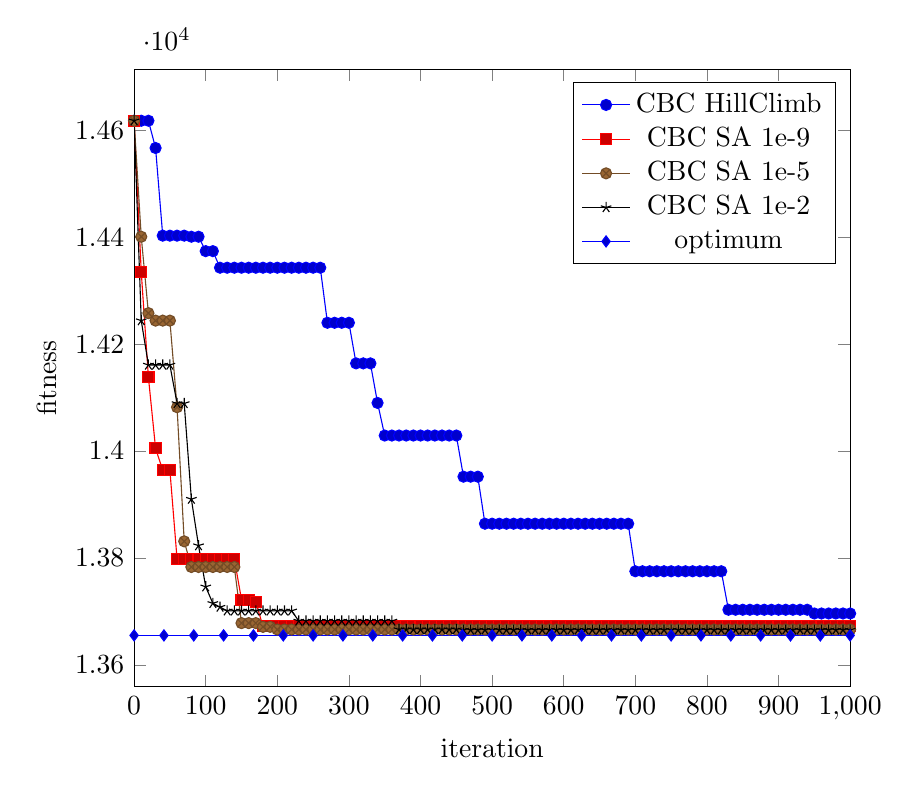
\begin{tikzpicture}
 \begin{axis}[
   width=0.75\textwidth,
   scale only axis,
   xlabel=iteration,
   ylabel=fitness,
   xmin=0,xmax=1000,
   domain=0:1000]
   \addplot coordinates {
     (0,14618)
     (10,14618)
     (20,14618)
     (30,14567)
     (40,14403)
     (50,14403)
     (60,14403)
     (70,14403)
     (80,14401)
     (90,14401)
     (100,14374)
     (110,14374)
     (120,14343)
     (130,14343)
     (140,14343)
     (150,14343)
     (160,14343)
     (170,14343)
     (180,14343)
     (190,14343)
     (200,14343)
     (210,14343)
     (220,14343)
     (230,14343)
     (240,14343)
     (250,14343)
     (260,14343)
     (270,14240)
     (280,14240)
     (290,14240)
     (300,14240)
     (310,14164)
     (320,14164)
     (330,14164)
     (340,14090)
     (350,14029)
     (360,14029)
     (370,14029)
     (380,14029)
     (390,14029)
     (400,14029)
     (410,14029)
     (420,14029)
     (430,14029)
     (440,14029)
     (450,14029)
     (460,13952)
     (470,13952)
     (480,13952)
     (490,13864)
     (500,13864)
     (510,13864)
     (520,13864)
     (530,13864)
     (540,13864)
     (550,13864)
     (560,13864)
     (570,13864)
     (580,13864)
     (590,13864)
     (600,13864)
     (610,13864)
     (620,13864)
     (630,13864)
     (640,13864)
     (650,13864)
     (660,13864)
     (670,13864)
     (680,13864)
     (690,13864)
     (700,13775)
     (710,13775)
     (720,13775)
     (730,13775)
     (740,13775)
     (750,13775)
     (760,13775)
     (770,13775)
     (780,13775)
     (790,13775)
     (800,13775)
     (810,13775)
     (820,13775)
     (830,13703)
     (840,13703)
     (850,13703)
     (860,13703)
     (870,13703)
     (880,13703)
     (890,13703)
     (900,13703)
     (910,13703)
     (920,13703)
     (930,13703)
     (940,13703)
     (950,13696)
     (960,13696)
     (970,13696)
     (980,13696)
     (990,13696)
     (1000,13696)
   };
   \addlegendentry{CBC HillClimb}
   \addplot coordinates {
     (0,14618)
     (10,14335)
     (20,14138)
     (30,14005)
     (40,13964)
     (50,13964)
     (60,13798)
     (70,13798)
     (80,13798)
     (90,13798)
     (100,13798)
     (110,13798)
     (120,13798)
     (130,13798)
     (140,13798)
     (150,13722)
     (160,13722)
     (170,13717)
     (180,13672)
     (190,13672)
     (200,13672)
     (210,13672)
     (220,13672)
     (230,13672)
     (240,13672)
     (250,13672)
     (260,13672)
     (270,13672)
     (280,13672)
     (290,13672)
     (300,13672)
     (310,13672)
     (320,13672)
     (330,13672)
     (340,13672)
     (350,13672)
     (360,13672)
     (370,13672)
     (380,13672)
     (390,13672)
     (400,13672)
     (410,13672)
     (420,13672)
     (430,13672)
     (440,13672)
     (450,13672)
     (460,13672)
     (470,13672)
     (480,13672)
     (490,13672)
     (500,13672)
     (510,13672)
     (520,13672)
     (530,13672)
     (540,13672)
     (550,13672)
     (560,13672)
     (570,13672)
     (580,13672)
     (590,13672)
     (600,13672)
     (610,13672)
     (620,13672)
     (630,13672)
     (640,13672)
     (650,13672)
     (660,13672)
     (670,13672)
     (680,13672)
     (690,13672)
     (700,13672)
     (710,13672)
     (720,13672)
     (730,13672)
     (740,13672)
     (750,13672)
     (760,13672)
     (770,13672)
     (780,13672)
     (790,13672)
     (800,13672)
     (810,13672)
     (820,13672)
     (830,13672)
     (840,13672)
     (850,13672)
     (860,13672)
     (870,13672)
     (880,13672)
     (890,13672)
     (900,13672)
     (910,13672)
     (920,13672)
     (930,13672)
     (940,13672)
     (950,13672)
     (960,13672)
     (970,13672)
     (980,13672)
     (990,13672)
     (1000,13672)
   };
   \addlegendentry{CBC SA 1e-9}
   \addplot coordinates {
     (0,14618)
     (10,14401)
     (20,14258)
     (30,14244)
     (40,14244)
     (50,14244)
     (60,14082)
     (70,13831)
     (80,13783)
     (90,13783)
     (100,13783)
     (110,13783)
     (120,13783)
     (130,13783)
     (140,13783)
     (150,13678)
     (160,13678)
     (170,13678)
     (180,13671)
     (190,13671)
     (200,13666)
     (210,13666)
     (220,13666)
     (230,13666)
     (240,13666)
     (250,13666)
     (260,13666)
     (270,13666)
     (280,13666)
     (290,13666)
     (300,13666)
     (310,13666)
     (320,13666)
     (330,13666)
     (340,13666)
     (350,13666)
     (360,13666)
     (370,13666)
     (380,13666)
     (390,13666)
     (400,13666)
     (410,13666)
     (420,13666)
     (430,13666)
     (440,13666)
     (450,13666)
     (460,13666)
     (470,13666)
     (480,13666)
     (490,13666)
     (500,13666)
     (510,13666)
     (520,13666)
     (530,13666)
     (540,13666)
     (550,13666)
     (560,13666)
     (570,13666)
     (580,13666)
     (590,13666)
     (600,13666)
     (610,13666)
     (620,13666)
     (630,13666)
     (640,13666)
     (650,13666)
     (660,13666)
     (670,13666)
     (680,13666)
     (690,13666)
     (700,13666)
     (710,13666)
     (720,13666)
     (730,13666)
     (740,13666)
     (750,13666)
     (760,13666)
     (770,13666)
     (780,13666)
     (790,13666)
     (800,13666)
     (810,13666)
     (820,13666)
     (830,13666)
     (840,13666)
     (850,13666)
     (860,13666)
     (870,13666)
     (880,13666)
     (890,13666)
     (900,13666)
     (910,13666)
     (920,13666)
     (930,13666)
     (940,13666)
     (950,13666)
     (960,13666)
     (970,13666)
     (980,13666)
     (990,13666)
     (1000,13666)
   };
   \addlegendentry{CBC SA 1e-5}
   \addplot coordinates {
     (0,14618)
     (10,14244)
     (20,14161)
     (30,14161)
     (40,14161)
     (50,14161)
     (60,14089)
     (70,14089)
     (80,13910)
     (90,13823)
     (100,13746)
     (110,13715)
     (120,13708)
     (130,13701)
     (140,13701)
     (150,13701)
     (160,13701)
     (170,13701)
     (180,13701)
     (190,13701)
     (200,13701)
     (210,13701)
     (220,13701)
     (230,13682)
     (240,13682)
     (250,13682)
     (260,13682)
     (270,13682)
     (280,13682)
     (290,13682)
     (300,13682)
     (310,13682)
     (320,13682)
     (330,13682)
     (340,13682)
     (350,13682)
     (360,13682)
     (370,13666)
     (380,13666)
     (390,13666)
     (400,13666)
     (410,13666)
     (420,13666)
     (430,13666)
     (440,13666)
     (450,13666)
     (460,13665)
     (470,13665)
     (480,13665)
     (490,13665)
     (500,13665)
     (510,13665)
     (520,13665)
     (530,13665)
     (540,13665)
     (550,13665)
     (560,13665)
     (570,13665)
     (580,13665)
     (590,13665)
     (600,13665)
     (610,13665)
     (620,13665)
     (630,13665)
     (640,13665)
     (650,13665)
     (660,13665)
     (670,13665)
     (680,13665)
     (690,13665)
     (700,13665)
     (710,13665)
     (720,13665)
     (730,13665)
     (740,13665)
     (750,13665)
     (760,13665)
     (770,13665)
     (780,13665)
     (790,13665)
     (800,13665)
     (810,13665)
     (820,13665)
     (830,13665)
     (840,13665)
     (850,13665)
     (860,13665)
     (870,13665)
     (880,13665)
     (890,13665)
     (900,13665)
     (910,13665)
     (920,13665)
     (930,13665)
     (940,13665)
     (950,13665)
     (960,13665)
     (970,13665)
     (980,13665)
     (990,13665)
     (1000,13665)
   };
   \addlegendentry{CBC SA 1e-2}
   \addplot {13655.000000};
   \addlegendentry{optimum}
 \end{axis}
 \end{tikzpicture}
\end{figure}

\pgfsetplotmarksize{0pt}
\begin{figure}
 \centering
 \caption{\label{CBC-c10}CBC-c10},
 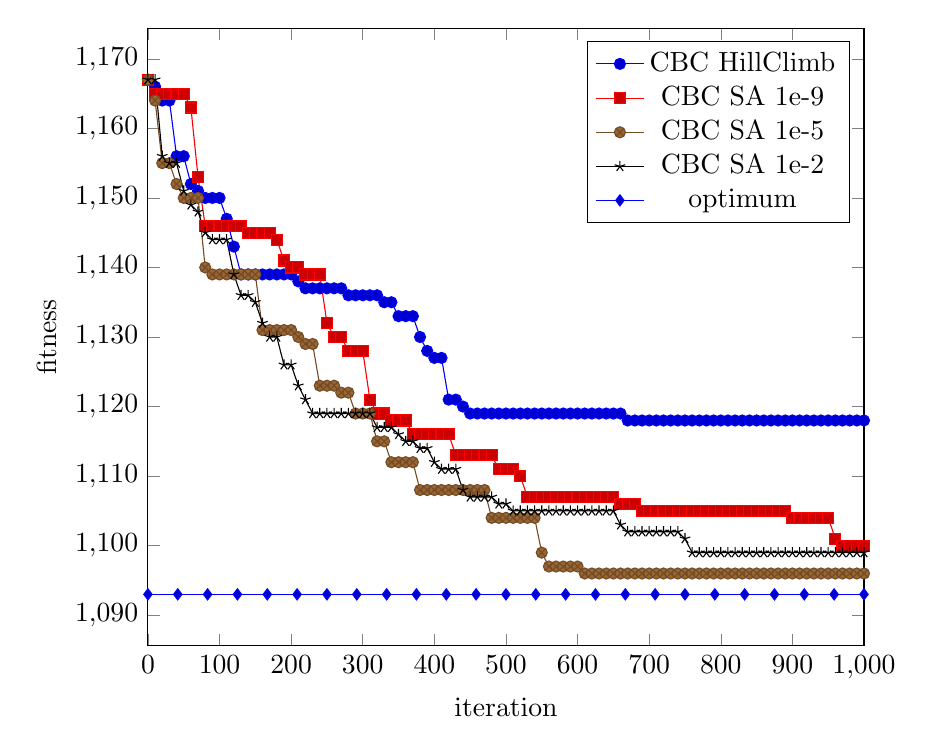
\begin{tikzpicture}
 \begin{axis}[
   width=0.75\textwidth,
   scale only axis,
   xlabel=iteration,
   ylabel=fitness,
   xmin=0,xmax=1000,
   domain=0:1000]
   \addplot coordinates {
     (0,1167)
     (10,1166)
     (20,1164)
     (30,1164)
     (40,1156)
     (50,1156)
     (60,1152)
     (70,1151)
     (80,1150)
     (90,1150)
     (100,1150)
     (110,1147)
     (120,1143)
     (130,1139)
     (140,1139)
     (150,1139)
     (160,1139)
     (170,1139)
     (180,1139)
     (190,1139)
     (200,1139)
     (210,1138)
     (220,1137)
     (230,1137)
     (240,1137)
     (250,1137)
     (260,1137)
     (270,1137)
     (280,1136)
     (290,1136)
     (300,1136)
     (310,1136)
     (320,1136)
     (330,1135)
     (340,1135)
     (350,1133)
     (360,1133)
     (370,1133)
     (380,1130)
     (390,1128)
     (400,1127)
     (410,1127)
     (420,1121)
     (430,1121)
     (440,1120)
     (450,1119)
     (460,1119)
     (470,1119)
     (480,1119)
     (490,1119)
     (500,1119)
     (510,1119)
     (520,1119)
     (530,1119)
     (540,1119)
     (550,1119)
     (560,1119)
     (570,1119)
     (580,1119)
     (590,1119)
     (600,1119)
     (610,1119)
     (620,1119)
     (630,1119)
     (640,1119)
     (650,1119)
     (660,1119)
     (670,1118)
     (680,1118)
     (690,1118)
     (700,1118)
     (710,1118)
     (720,1118)
     (730,1118)
     (740,1118)
     (750,1118)
     (760,1118)
     (770,1118)
     (780,1118)
     (790,1118)
     (800,1118)
     (810,1118)
     (820,1118)
     (830,1118)
     (840,1118)
     (850,1118)
     (860,1118)
     (870,1118)
     (880,1118)
     (890,1118)
     (900,1118)
     (910,1118)
     (920,1118)
     (930,1118)
     (940,1118)
     (950,1118)
     (960,1118)
     (970,1118)
     (980,1118)
     (990,1118)
     (1000,1118)
   };
   \addlegendentry{CBC HillClimb}
   \addplot coordinates {
     (0,1167)
     (10,1165)
     (20,1165)
     (30,1165)
     (40,1165)
     (50,1165)
     (60,1163)
     (70,1153)
     (80,1146)
     (90,1146)
     (100,1146)
     (110,1146)
     (120,1146)
     (130,1146)
     (140,1145)
     (150,1145)
     (160,1145)
     (170,1145)
     (180,1144)
     (190,1141)
     (200,1140)
     (210,1140)
     (220,1139)
     (230,1139)
     (240,1139)
     (250,1132)
     (260,1130)
     (270,1130)
     (280,1128)
     (290,1128)
     (300,1128)
     (310,1121)
     (320,1119)
     (330,1119)
     (340,1118)
     (350,1118)
     (360,1118)
     (370,1116)
     (380,1116)
     (390,1116)
     (400,1116)
     (410,1116)
     (420,1116)
     (430,1113)
     (440,1113)
     (450,1113)
     (460,1113)
     (470,1113)
     (480,1113)
     (490,1111)
     (500,1111)
     (510,1111)
     (520,1110)
     (530,1107)
     (540,1107)
     (550,1107)
     (560,1107)
     (570,1107)
     (580,1107)
     (590,1107)
     (600,1107)
     (610,1107)
     (620,1107)
     (630,1107)
     (640,1107)
     (650,1107)
     (660,1106)
     (670,1106)
     (680,1106)
     (690,1105)
     (700,1105)
     (710,1105)
     (720,1105)
     (730,1105)
     (740,1105)
     (750,1105)
     (760,1105)
     (770,1105)
     (780,1105)
     (790,1105)
     (800,1105)
     (810,1105)
     (820,1105)
     (830,1105)
     (840,1105)
     (850,1105)
     (860,1105)
     (870,1105)
     (880,1105)
     (890,1105)
     (900,1104)
     (910,1104)
     (920,1104)
     (930,1104)
     (940,1104)
     (950,1104)
     (960,1101)
     (970,1100)
     (980,1100)
     (990,1100)
     (1000,1100)
   };
   \addlegendentry{CBC SA 1e-9}
   \addplot coordinates {
     (0,1167)
     (10,1164)
     (20,1155)
     (30,1155)
     (40,1152)
     (50,1150)
     (60,1150)
     (70,1150)
     (80,1140)
     (90,1139)
     (100,1139)
     (110,1139)
     (120,1139)
     (130,1139)
     (140,1139)
     (150,1139)
     (160,1131)
     (170,1131)
     (180,1131)
     (190,1131)
     (200,1131)
     (210,1130)
     (220,1129)
     (230,1129)
     (240,1123)
     (250,1123)
     (260,1123)
     (270,1122)
     (280,1122)
     (290,1119)
     (300,1119)
     (310,1119)
     (320,1115)
     (330,1115)
     (340,1112)
     (350,1112)
     (360,1112)
     (370,1112)
     (380,1108)
     (390,1108)
     (400,1108)
     (410,1108)
     (420,1108)
     (430,1108)
     (440,1108)
     (450,1108)
     (460,1108)
     (470,1108)
     (480,1104)
     (490,1104)
     (500,1104)
     (510,1104)
     (520,1104)
     (530,1104)
     (540,1104)
     (550,1099)
     (560,1097)
     (570,1097)
     (580,1097)
     (590,1097)
     (600,1097)
     (610,1096)
     (620,1096)
     (630,1096)
     (640,1096)
     (650,1096)
     (660,1096)
     (670,1096)
     (680,1096)
     (690,1096)
     (700,1096)
     (710,1096)
     (720,1096)
     (730,1096)
     (740,1096)
     (750,1096)
     (760,1096)
     (770,1096)
     (780,1096)
     (790,1096)
     (800,1096)
     (810,1096)
     (820,1096)
     (830,1096)
     (840,1096)
     (850,1096)
     (860,1096)
     (870,1096)
     (880,1096)
     (890,1096)
     (900,1096)
     (910,1096)
     (920,1096)
     (930,1096)
     (940,1096)
     (950,1096)
     (960,1096)
     (970,1096)
     (980,1096)
     (990,1096)
     (1000,1096)
   };
   \addlegendentry{CBC SA 1e-5}
   \addplot coordinates {
     (0,1167)
     (10,1167)
     (20,1156)
     (30,1155)
     (40,1155)
     (50,1151)
     (60,1149)
     (70,1148)
     (80,1145)
     (90,1144)
     (100,1144)
     (110,1144)
     (120,1139)
     (130,1136)
     (140,1136)
     (150,1135)
     (160,1132)
     (170,1130)
     (180,1130)
     (190,1126)
     (200,1126)
     (210,1123)
     (220,1121)
     (230,1119)
     (240,1119)
     (250,1119)
     (260,1119)
     (270,1119)
     (280,1119)
     (290,1119)
     (300,1119)
     (310,1119)
     (320,1117)
     (330,1117)
     (340,1117)
     (350,1116)
     (360,1115)
     (370,1115)
     (380,1114)
     (390,1114)
     (400,1112)
     (410,1111)
     (420,1111)
     (430,1111)
     (440,1108)
     (450,1107)
     (460,1107)
     (470,1107)
     (480,1107)
     (490,1106)
     (500,1106)
     (510,1105)
     (520,1105)
     (530,1105)
     (540,1105)
     (550,1105)
     (560,1105)
     (570,1105)
     (580,1105)
     (590,1105)
     (600,1105)
     (610,1105)
     (620,1105)
     (630,1105)
     (640,1105)
     (650,1105)
     (660,1103)
     (670,1102)
     (680,1102)
     (690,1102)
     (700,1102)
     (710,1102)
     (720,1102)
     (730,1102)
     (740,1102)
     (750,1101)
     (760,1099)
     (770,1099)
     (780,1099)
     (790,1099)
     (800,1099)
     (810,1099)
     (820,1099)
     (830,1099)
     (840,1099)
     (850,1099)
     (860,1099)
     (870,1099)
     (880,1099)
     (890,1099)
     (900,1099)
     (910,1099)
     (920,1099)
     (930,1099)
     (940,1099)
     (950,1099)
     (960,1099)
     (970,1099)
     (980,1099)
     (990,1099)
     (1000,1099)
   };
   \addlegendentry{CBC SA 1e-2}
   \addplot {1093.000000};
   \addlegendentry{optimum}
 \end{axis}
 \end{tikzpicture}
\end{figure}


\pgfsetplotmarksize{0pt}
 \centering
 \caption{\label{MSTAV-01dEV100K30}MSTAV-01dEV100K30},
 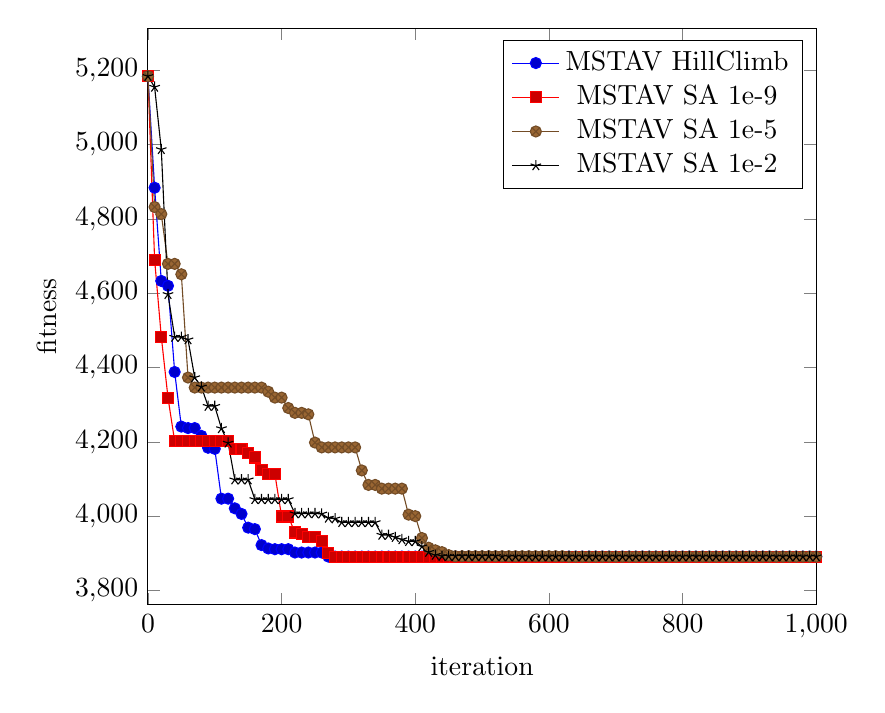
\begin{tikzpicture}
 \begin{axis}[
   width=0.7\textwidth,
   scale only axis,
   xlabel=iteration,
   ylabel=fitness,
   xmin=0,xmax=1000,
   domain=0:1000]
   \addplot coordinates {
     (0,5184)
     (10,4884)
     (20,4633)
     (30,4620)
     (40,4388)
     (50,4241)
     (60,4237)
     (70,4237)
     (80,4216)
     (90,4184)
     (100,4181)
     (110,4047)
     (120,4047)
     (130,4021)
     (140,4006)
     (150,3969)
     (160,3965)
     (170,3922)
     (180,3913)
     (190,3911)
     (200,3911)
     (210,3911)
     (220,3902)
     (230,3902)
     (240,3902)
     (250,3902)
     (260,3902)
     (270,3891)
     (280,3891)
     (290,3891)
     (300,3891)
     (310,3891)
     (320,3891)
     (330,3891)
     (340,3891)
     (350,3891)
     (360,3891)
     (370,3891)
     (380,3891)
     (390,3891)
     (400,3891)
     (410,3891)
     (420,3891)
     (430,3891)
     (440,3891)
     (450,3891)
     (460,3891)
     (470,3891)
     (480,3891)
     (490,3891)
     (500,3891)
     (510,3891)
     (520,3891)
     (530,3891)
     (540,3891)
     (550,3891)
     (560,3891)
     (570,3891)
     (580,3891)
     (590,3891)
     (600,3891)
     (610,3891)
     (620,3891)
     (630,3891)
     (640,3891)
     (650,3891)
     (660,3891)
     (670,3891)
     (680,3891)
     (690,3891)
     (700,3891)
     (710,3891)
     (720,3891)
     (730,3891)
     (740,3891)
     (750,3891)
     (760,3891)
     (770,3891)
     (780,3891)
     (790,3891)
     (800,3891)
     (810,3891)
     (820,3891)
     (830,3891)
     (840,3891)
     (850,3891)
     (860,3891)
     (870,3891)
     (880,3891)
     (890,3891)
     (900,3891)
     (910,3891)
     (920,3891)
     (930,3891)
     (940,3891)
     (950,3891)
     (960,3891)
     (970,3891)
     (980,3891)
     (990,3891)
     (1000,3891)
   };
   \addlegendentry{MSTAV HillClimb}
   \addplot coordinates {
     (0,5184)
     (10,4690)
     (20,4483)
     (30,4319)
     (40,4202)
     (50,4202)
     (60,4202)
     (70,4202)
     (80,4202)
     (90,4202)
     (100,4202)
     (110,4202)
     (120,4202)
     (130,4180)
     (140,4180)
     (150,4169)
     (160,4158)
     (170,4125)
     (180,4113)
     (190,4113)
     (200,3999)
     (210,3999)
     (220,3956)
     (230,3952)
     (240,3944)
     (250,3944)
     (260,3933)
     (270,3901)
     (280,3891)
     (290,3891)
     (300,3891)
     (310,3891)
     (320,3891)
     (330,3891)
     (340,3891)
     (350,3891)
     (360,3891)
     (370,3891)
     (380,3891)
     (390,3891)
     (400,3891)
     (410,3891)
     (420,3891)
     (430,3891)
     (440,3891)
     (450,3891)
     (460,3891)
     (470,3891)
     (480,3891)
     (490,3891)
     (500,3891)
     (510,3891)
     (520,3891)
     (530,3891)
     (540,3891)
     (550,3891)
     (560,3891)
     (570,3891)
     (580,3891)
     (590,3891)
     (600,3891)
     (610,3891)
     (620,3891)
     (630,3891)
     (640,3891)
     (650,3891)
     (660,3891)
     (670,3891)
     (680,3891)
     (690,3891)
     (700,3891)
     (710,3891)
     (720,3891)
     (730,3891)
     (740,3891)
     (750,3891)
     (760,3891)
     (770,3891)
     (780,3891)
     (790,3891)
     (800,3891)
     (810,3891)
     (820,3891)
     (830,3891)
     (840,3891)
     (850,3891)
     (860,3891)
     (870,3891)
     (880,3891)
     (890,3891)
     (900,3891)
     (910,3891)
     (920,3891)
     (930,3891)
     (940,3891)
     (950,3891)
     (960,3891)
     (970,3891)
     (980,3891)
     (990,3891)
     (1000,3891)
   };
   \addlegendentry{MSTAV SA 1e-9}
   \addplot coordinates {
     (0,5184)
     (10,4832)
     (20,4813)
     (30,4679)
     (40,4679)
     (50,4651)
     (60,4373)
     (70,4346)
     (80,4346)
     (90,4346)
     (100,4346)
     (110,4346)
     (120,4346)
     (130,4346)
     (140,4346)
     (150,4346)
     (160,4346)
     (170,4346)
     (180,4335)
     (190,4319)
     (200,4319)
     (210,4291)
     (220,4278)
     (230,4278)
     (240,4274)
     (250,4198)
     (260,4185)
     (270,4185)
     (280,4185)
     (290,4185)
     (300,4185)
     (310,4185)
     (320,4123)
     (330,4084)
     (340,4084)
     (350,4074)
     (360,4074)
     (370,4074)
     (380,4074)
     (390,4004)
     (400,4000)
     (410,3941)
     (420,3915)
     (430,3908)
     (440,3903)
     (450,3895)
     (460,3892)
     (470,3892)
     (480,3892)
     (490,3892)
     (500,3892)
     (510,3892)
     (520,3892)
     (530,3892)
     (540,3892)
     (550,3892)
     (560,3892)
     (570,3892)
     (580,3892)
     (590,3892)
     (600,3892)
     (610,3892)
     (620,3892)
     (630,3891)
     (640,3891)
     (650,3891)
     (660,3891)
     (670,3891)
     (680,3891)
     (690,3891)
     (700,3891)
     (710,3891)
     (720,3891)
     (730,3891)
     (740,3891)
     (750,3891)
     (760,3891)
     (770,3891)
     (780,3891)
     (790,3891)
     (800,3891)
     (810,3891)
     (820,3891)
     (830,3891)
     (840,3891)
     (850,3891)
     (860,3891)
     (870,3891)
     (880,3891)
     (890,3891)
     (900,3891)
     (910,3891)
     (920,3891)
     (930,3891)
     (940,3891)
     (950,3891)
     (960,3891)
     (970,3891)
     (980,3891)
     (990,3891)
     (1000,3891)
   };
   \addlegendentry{MSTAV SA 1e-5}
   \addplot coordinates {
     (0,5184)
     (10,5155)
     (20,4987)
     (30,4597)
     (40,4482)
     (50,4482)
     (60,4475)
     (70,4373)
     (80,4348)
     (90,4296)
     (100,4296)
     (110,4236)
     (120,4197)
     (130,4098)
     (140,4098)
     (150,4098)
     (160,4045)
     (170,4045)
     (180,4045)
     (190,4045)
     (200,4045)
     (210,4045)
     (220,4007)
     (230,4007)
     (240,4007)
     (250,4007)
     (260,4006)
     (270,3995)
     (280,3993)
     (290,3983)
     (300,3983)
     (310,3983)
     (320,3983)
     (330,3983)
     (340,3983)
     (350,3949)
     (360,3949)
     (370,3943)
     (380,3937)
     (390,3932)
     (400,3932)
     (410,3918)
     (420,3903)
     (430,3895)
     (440,3892)
     (450,3892)
     (460,3892)
     (470,3892)
     (480,3892)
     (490,3892)
     (500,3892)
     (510,3892)
     (520,3892)
     (530,3891)
     (540,3891)
     (550,3891)
     (560,3891)
     (570,3891)
     (580,3891)
     (590,3891)
     (600,3891)
     (610,3891)
     (620,3891)
     (630,3891)
     (640,3891)
     (650,3891)
     (660,3891)
     (670,3891)
     (680,3891)
     (690,3891)
     (700,3891)
     (710,3891)
     (720,3891)
     (730,3891)
     (740,3891)
     (750,3891)
     (760,3891)
     (770,3891)
     (780,3891)
     (790,3891)
     (800,3891)
     (810,3891)
     (820,3891)
     (830,3891)
     (840,3891)
     (850,3891)
     (860,3891)
     (870,3891)
     (880,3891)
     (890,3891)
     (900,3891)
     (910,3891)
     (920,3891)
     (930,3891)
     (940,3891)
     (950,3891)
     (960,3891)
     (970,3891)
     (980,3891)
     (990,3891)
     (1000,3891)
   };
   \addlegendentry{MSTAV SA 1e-2}
 \end{axis}
 \end{tikzpicture}

\pgfsetplotmarksize{0pt}
 \centering
 \caption{\label{MSTAV-02dEV100K30}MSTAV-02dEV100K30},
 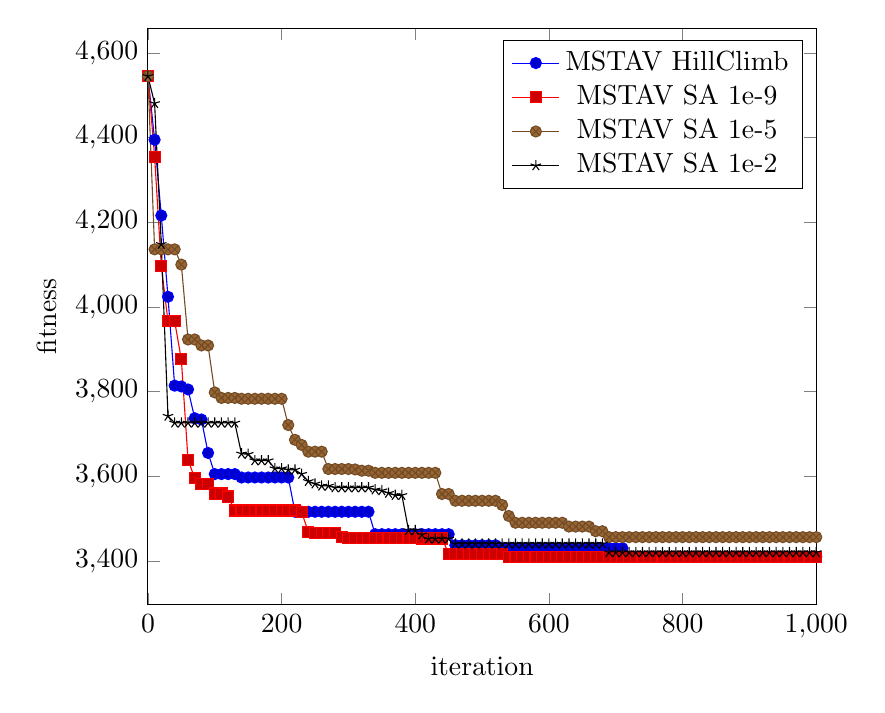
\begin{tikzpicture}
 \begin{axis}[
   width=0.7\textwidth,
   scale only axis,
   xlabel=iteration,
   ylabel=fitness,
   xmin=0,xmax=1000,
   domain=0:1000]
   \addplot coordinates {
     (0,4545)
     (10,4395)
     (20,4216)
     (30,4024)
     (40,3814)
     (50,3812)
     (60,3805)
     (70,3737)
     (80,3734)
     (90,3655)
     (100,3605)
     (110,3605)
     (120,3605)
     (130,3605)
     (140,3597)
     (150,3597)
     (160,3597)
     (170,3597)
     (180,3597)
     (190,3597)
     (200,3597)
     (210,3597)
     (220,3516)
     (230,3516)
     (240,3516)
     (250,3516)
     (260,3516)
     (270,3516)
     (280,3516)
     (290,3516)
     (300,3516)
     (310,3516)
     (320,3516)
     (330,3516)
     (340,3463)
     (350,3463)
     (360,3463)
     (370,3463)
     (380,3463)
     (390,3463)
     (400,3463)
     (410,3463)
     (420,3463)
     (430,3463)
     (440,3463)
     (450,3463)
     (460,3437)
     (470,3437)
     (480,3437)
     (490,3437)
     (500,3437)
     (510,3437)
     (520,3437)
     (530,3430)
     (540,3430)
     (550,3430)
     (560,3430)
     (570,3430)
     (580,3430)
     (590,3430)
     (600,3430)
     (610,3430)
     (620,3430)
     (630,3430)
     (640,3430)
     (650,3430)
     (660,3430)
     (670,3430)
     (680,3430)
     (690,3430)
     (700,3430)
     (710,3430)
     (720,3410)
     (730,3410)
     (740,3410)
     (750,3410)
     (760,3410)
     (770,3410)
     (780,3410)
     (790,3410)
     (800,3410)
     (810,3410)
     (820,3410)
     (830,3410)
     (840,3410)
     (850,3410)
     (860,3410)
     (870,3410)
     (880,3410)
     (890,3410)
     (900,3410)
     (910,3410)
     (920,3410)
     (930,3410)
     (940,3410)
     (950,3410)
     (960,3410)
     (970,3410)
     (980,3410)
     (990,3410)
     (1000,3410)
   };
   \addlegendentry{MSTAV HillClimb}
   \addplot coordinates {
     (0,4545)
     (10,4355)
     (20,4097)
     (30,3966)
     (40,3966)
     (50,3876)
     (60,3639)
     (70,3595)
     (80,3581)
     (90,3581)
     (100,3559)
     (110,3559)
     (120,3552)
     (130,3519)
     (140,3519)
     (150,3519)
     (160,3519)
     (170,3519)
     (180,3519)
     (190,3519)
     (200,3519)
     (210,3519)
     (220,3519)
     (230,3515)
     (240,3468)
     (250,3465)
     (260,3465)
     (270,3465)
     (280,3465)
     (290,3457)
     (300,3454)
     (310,3454)
     (320,3454)
     (330,3454)
     (340,3454)
     (350,3454)
     (360,3454)
     (370,3454)
     (380,3454)
     (390,3454)
     (400,3454)
     (410,3453)
     (420,3453)
     (430,3453)
     (440,3453)
     (450,3417)
     (460,3417)
     (470,3417)
     (480,3417)
     (490,3417)
     (500,3417)
     (510,3417)
     (520,3417)
     (530,3417)
     (540,3410)
     (550,3410)
     (560,3410)
     (570,3410)
     (580,3410)
     (590,3410)
     (600,3410)
     (610,3410)
     (620,3410)
     (630,3410)
     (640,3410)
     (650,3410)
     (660,3410)
     (670,3410)
     (680,3410)
     (690,3410)
     (700,3410)
     (710,3410)
     (720,3410)
     (730,3410)
     (740,3410)
     (750,3410)
     (760,3410)
     (770,3410)
     (780,3410)
     (790,3410)
     (800,3410)
     (810,3410)
     (820,3410)
     (830,3410)
     (840,3410)
     (850,3410)
     (860,3410)
     (870,3410)
     (880,3410)
     (890,3410)
     (900,3410)
     (910,3410)
     (920,3410)
     (930,3410)
     (940,3410)
     (950,3410)
     (960,3410)
     (970,3410)
     (980,3410)
     (990,3410)
     (1000,3410)
   };
   \addlegendentry{MSTAV SA 1e-9}
   \addplot coordinates {
     (0,4545)
     (10,4136)
     (20,4136)
     (30,4136)
     (40,4136)
     (50,4100)
     (60,3923)
     (70,3923)
     (80,3909)
     (90,3909)
     (100,3798)
     (110,3785)
     (120,3785)
     (130,3785)
     (140,3783)
     (150,3783)
     (160,3783)
     (170,3783)
     (180,3783)
     (190,3783)
     (200,3783)
     (210,3721)
     (220,3686)
     (230,3674)
     (240,3658)
     (250,3658)
     (260,3658)
     (270,3617)
     (280,3617)
     (290,3617)
     (300,3617)
     (310,3616)
     (320,3613)
     (330,3613)
     (340,3608)
     (350,3608)
     (360,3608)
     (370,3608)
     (380,3608)
     (390,3608)
     (400,3608)
     (410,3608)
     (420,3608)
     (430,3608)
     (440,3558)
     (450,3558)
     (460,3542)
     (470,3542)
     (480,3542)
     (490,3542)
     (500,3542)
     (510,3542)
     (520,3542)
     (530,3532)
     (540,3506)
     (550,3490)
     (560,3490)
     (570,3490)
     (580,3490)
     (590,3490)
     (600,3490)
     (610,3490)
     (620,3490)
     (630,3481)
     (640,3481)
     (650,3481)
     (660,3481)
     (670,3470)
     (680,3470)
     (690,3456)
     (700,3456)
     (710,3456)
     (720,3456)
     (730,3456)
     (740,3456)
     (750,3456)
     (760,3456)
     (770,3456)
     (780,3456)
     (790,3456)
     (800,3456)
     (810,3456)
     (820,3456)
     (830,3456)
     (840,3456)
     (850,3456)
     (860,3456)
     (870,3456)
     (880,3456)
     (890,3456)
     (900,3456)
     (910,3456)
     (920,3456)
     (930,3456)
     (940,3456)
     (950,3456)
     (960,3456)
     (970,3456)
     (980,3456)
     (990,3456)
     (1000,3456)
   };
   \addlegendentry{MSTAV SA 1e-5}
   \addplot coordinates {
     (0,4545)
     (10,4481)
     (20,4148)
     (30,3742)
     (40,3726)
     (50,3726)
     (60,3726)
     (70,3726)
     (80,3726)
     (90,3726)
     (100,3726)
     (110,3726)
     (120,3726)
     (130,3726)
     (140,3653)
     (150,3652)
     (160,3637)
     (170,3637)
     (180,3637)
     (190,3618)
     (200,3618)
     (210,3615)
     (220,3615)
     (230,3605)
     (240,3588)
     (250,3582)
     (260,3577)
     (270,3577)
     (280,3573)
     (290,3573)
     (300,3573)
     (310,3573)
     (320,3573)
     (330,3573)
     (340,3568)
     (350,3566)
     (360,3560)
     (370,3555)
     (380,3555)
     (390,3472)
     (400,3472)
     (410,3462)
     (420,3452)
     (430,3452)
     (440,3452)
     (450,3452)
     (460,3440)
     (470,3440)
     (480,3440)
     (490,3440)
     (500,3440)
     (510,3440)
     (520,3440)
     (530,3440)
     (540,3440)
     (550,3440)
     (560,3440)
     (570,3440)
     (580,3440)
     (590,3440)
     (600,3440)
     (610,3440)
     (620,3440)
     (630,3440)
     (640,3440)
     (650,3440)
     (660,3440)
     (670,3440)
     (680,3440)
     (690,3420)
     (700,3420)
     (710,3420)
     (720,3420)
     (730,3420)
     (740,3420)
     (750,3420)
     (760,3420)
     (770,3420)
     (780,3420)
     (790,3420)
     (800,3420)
     (810,3420)
     (820,3420)
     (830,3420)
     (840,3420)
     (850,3420)
     (860,3420)
     (870,3420)
     (880,3420)
     (890,3420)
     (900,3420)
     (910,3420)
     (920,3420)
     (930,3420)
     (940,3420)
     (950,3420)
     (960,3420)
     (970,3420)
     (980,3420)
     (990,3420)
     (1000,3420)
   };
   \addlegendentry{MSTAV SA 1e-2}
 \end{axis}
 \end{tikzpicture}

\pgfsetplotmarksize{0pt}
\begin{figure}
 \centering
 \caption{\label{MSTAV-alue2087}MSTAV-alue2087},
 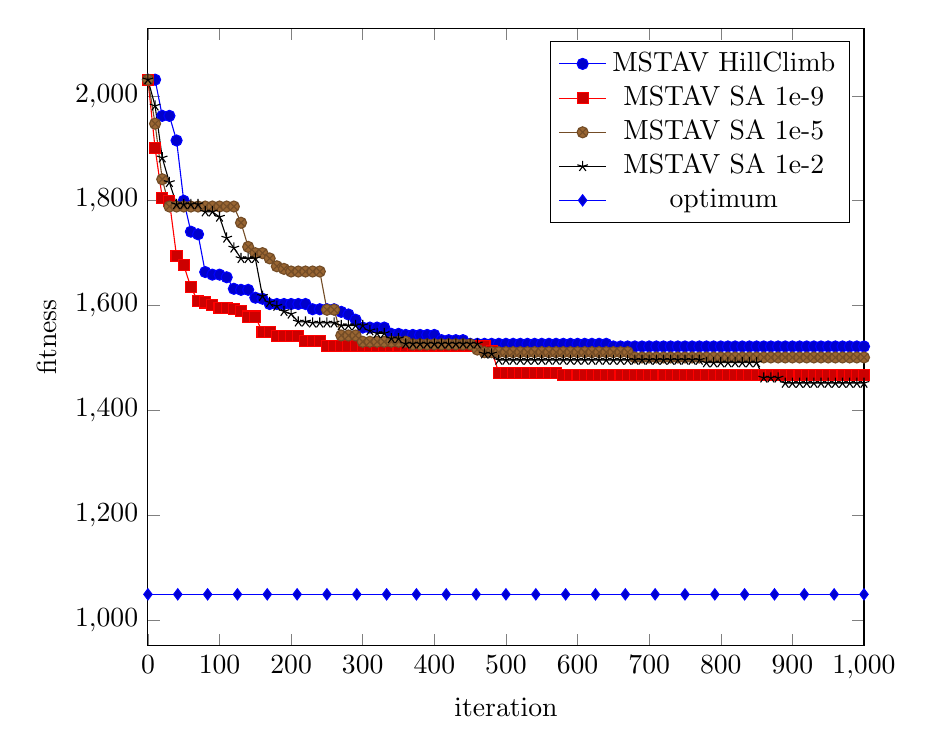
\begin{tikzpicture}
 \begin{axis}[
   width=0.75\textwidth,
   scale only axis,
   xlabel=iteration,
   ylabel=fitness,
   xmin=0,xmax=1000,
   domain=0:1000]
   \addplot coordinates {
     (0,2031)
     (10,2031)
     (20,1962)
     (30,1962)
     (40,1915)
     (50,1800)
     (60,1741)
     (70,1736)
     (80,1664)
     (90,1659)
     (100,1659)
     (110,1654)
     (120,1632)
     (130,1630)
     (140,1630)
     (150,1615)
     (160,1613)
     (170,1603)
     (180,1603)
     (190,1603)
     (200,1603)
     (210,1603)
     (220,1603)
     (230,1593)
     (240,1593)
     (250,1593)
     (260,1593)
     (270,1588)
     (280,1583)
     (290,1573)
     (300,1558)
     (310,1558)
     (320,1558)
     (330,1558)
     (340,1546)
     (350,1546)
     (360,1544)
     (370,1544)
     (380,1544)
     (390,1544)
     (400,1544)
     (410,1534)
     (420,1534)
     (430,1534)
     (440,1534)
     (450,1527)
     (460,1527)
     (470,1527)
     (480,1527)
     (490,1527)
     (500,1527)
     (510,1527)
     (520,1527)
     (530,1527)
     (540,1527)
     (550,1527)
     (560,1527)
     (570,1527)
     (580,1527)
     (590,1527)
     (600,1527)
     (610,1527)
     (620,1527)
     (630,1527)
     (640,1527)
     (650,1522)
     (660,1522)
     (670,1522)
     (680,1522)
     (690,1522)
     (700,1522)
     (710,1522)
     (720,1522)
     (730,1522)
     (740,1522)
     (750,1522)
     (760,1522)
     (770,1522)
     (780,1522)
     (790,1522)
     (800,1522)
     (810,1522)
     (820,1522)
     (830,1522)
     (840,1522)
     (850,1522)
     (860,1522)
     (870,1522)
     (880,1522)
     (890,1522)
     (900,1522)
     (910,1522)
     (920,1522)
     (930,1522)
     (940,1522)
     (950,1522)
     (960,1522)
     (970,1522)
     (980,1522)
     (990,1522)
     (1000,1522)
   };
   \addlegendentry{MSTAV HillClimb}
   \addplot coordinates {
     (0,2031)
     (10,1900)
     (20,1806)
     (30,1799)
     (40,1694)
     (50,1677)
     (60,1635)
     (70,1608)
     (80,1606)
     (90,1601)
     (100,1596)
     (110,1596)
     (120,1594)
     (130,1589)
     (140,1579)
     (150,1579)
     (160,1549)
     (170,1549)
     (180,1542)
     (190,1542)
     (200,1542)
     (210,1542)
     (220,1532)
     (230,1532)
     (240,1532)
     (250,1523)
     (260,1523)
     (270,1523)
     (280,1523)
     (290,1523)
     (300,1523)
     (310,1523)
     (320,1523)
     (330,1523)
     (340,1523)
     (350,1523)
     (360,1523)
     (370,1523)
     (380,1523)
     (390,1523)
     (400,1523)
     (410,1523)
     (420,1523)
     (430,1523)
     (440,1523)
     (450,1523)
     (460,1523)
     (470,1523)
     (480,1513)
     (490,1472)
     (500,1472)
     (510,1472)
     (520,1472)
     (530,1472)
     (540,1472)
     (550,1472)
     (560,1472)
     (570,1472)
     (580,1467)
     (590,1467)
     (600,1467)
     (610,1467)
     (620,1467)
     (630,1467)
     (640,1467)
     (650,1467)
     (660,1467)
     (670,1467)
     (680,1467)
     (690,1467)
     (700,1467)
     (710,1467)
     (720,1467)
     (730,1467)
     (740,1467)
     (750,1467)
     (760,1467)
     (770,1467)
     (780,1467)
     (790,1467)
     (800,1467)
     (810,1467)
     (820,1467)
     (830,1467)
     (840,1467)
     (850,1467)
     (860,1467)
     (870,1467)
     (880,1467)
     (890,1467)
     (900,1467)
     (910,1467)
     (920,1467)
     (930,1467)
     (940,1467)
     (950,1467)
     (960,1467)
     (970,1467)
     (980,1467)
     (990,1467)
     (1000,1467)
   };
   \addlegendentry{MSTAV SA 1e-9}
   \addplot coordinates {
     (0,2031)
     (10,1947)
     (20,1841)
     (30,1789)
     (40,1789)
     (50,1789)
     (60,1789)
     (70,1789)
     (80,1789)
     (90,1789)
     (100,1789)
     (110,1789)
     (120,1789)
     (130,1758)
     (140,1712)
     (150,1700)
     (160,1700)
     (170,1690)
     (180,1675)
     (190,1670)
     (200,1665)
     (210,1665)
     (220,1665)
     (230,1665)
     (240,1665)
     (250,1592)
     (260,1592)
     (270,1543)
     (280,1543)
     (290,1543)
     (300,1531)
     (310,1531)
     (320,1531)
     (330,1531)
     (340,1531)
     (350,1531)
     (360,1531)
     (370,1526)
     (380,1526)
     (390,1526)
     (400,1526)
     (410,1526)
     (420,1526)
     (430,1526)
     (440,1526)
     (450,1526)
     (460,1516)
     (470,1511)
     (480,1511)
     (490,1511)
     (500,1511)
     (510,1511)
     (520,1511)
     (530,1511)
     (540,1511)
     (550,1511)
     (560,1511)
     (570,1511)
     (580,1511)
     (590,1511)
     (600,1511)
     (610,1511)
     (620,1511)
     (630,1511)
     (640,1511)
     (650,1511)
     (660,1511)
     (670,1511)
     (680,1501)
     (690,1501)
     (700,1501)
     (710,1501)
     (720,1501)
     (730,1501)
     (740,1501)
     (750,1501)
     (760,1501)
     (770,1501)
     (780,1501)
     (790,1501)
     (800,1501)
     (810,1501)
     (820,1501)
     (830,1501)
     (840,1501)
     (850,1501)
     (860,1501)
     (870,1501)
     (880,1501)
     (890,1501)
     (900,1501)
     (910,1501)
     (920,1501)
     (930,1501)
     (940,1501)
     (950,1501)
     (960,1501)
     (970,1501)
     (980,1501)
     (990,1501)
     (1000,1501)
   };
   \addlegendentry{MSTAV SA 1e-5}
   \addplot coordinates {
     (0,2031)
     (10,1981)
     (20,1882)
     (30,1835)
     (40,1793)
     (50,1793)
     (60,1793)
     (70,1793)
     (80,1779)
     (90,1779)
     (100,1769)
     (110,1729)
     (120,1710)
     (130,1690)
     (140,1690)
     (150,1690)
     (160,1618)
     (170,1606)
     (180,1599)
     (190,1589)
     (200,1584)
     (210,1569)
     (220,1569)
     (230,1567)
     (240,1567)
     (250,1567)
     (260,1567)
     (270,1562)
     (280,1562)
     (290,1562)
     (300,1562)
     (310,1552)
     (320,1547)
     (330,1547)
     (340,1537)
     (350,1537)
     (360,1527)
     (370,1527)
     (380,1527)
     (390,1527)
     (400,1527)
     (410,1527)
     (420,1527)
     (430,1527)
     (440,1527)
     (450,1527)
     (460,1527)
     (470,1508)
     (480,1508)
     (490,1496)
     (500,1496)
     (510,1496)
     (520,1496)
     (530,1496)
     (540,1496)
     (550,1496)
     (560,1496)
     (570,1496)
     (580,1496)
     (590,1496)
     (600,1496)
     (610,1496)
     (620,1496)
     (630,1496)
     (640,1496)
     (650,1496)
     (660,1496)
     (670,1496)
     (680,1496)
     (690,1496)
     (700,1496)
     (710,1496)
     (720,1496)
     (730,1496)
     (740,1496)
     (750,1496)
     (760,1496)
     (770,1496)
     (780,1491)
     (790,1491)
     (800,1491)
     (810,1491)
     (820,1491)
     (830,1491)
     (840,1491)
     (850,1491)
     (860,1462)
     (870,1462)
     (880,1462)
     (890,1452)
     (900,1452)
     (910,1452)
     (920,1452)
     (930,1452)
     (940,1452)
     (950,1452)
     (960,1452)
     (970,1452)
     (980,1452)
     (990,1452)
     (1000,1452)
   };
   \addlegendentry{MSTAV SA 1e-2}
   \addplot {1049.000000};
   \addlegendentry{optimum}
 \end{axis}
 \end{tikzpicture}
\end{figure}

\pgfsetplotmarksize{0pt}
\begin{figure}
 \centering
 \caption{\label{MSTAV-berlin52}MSTAV-berlin52},
 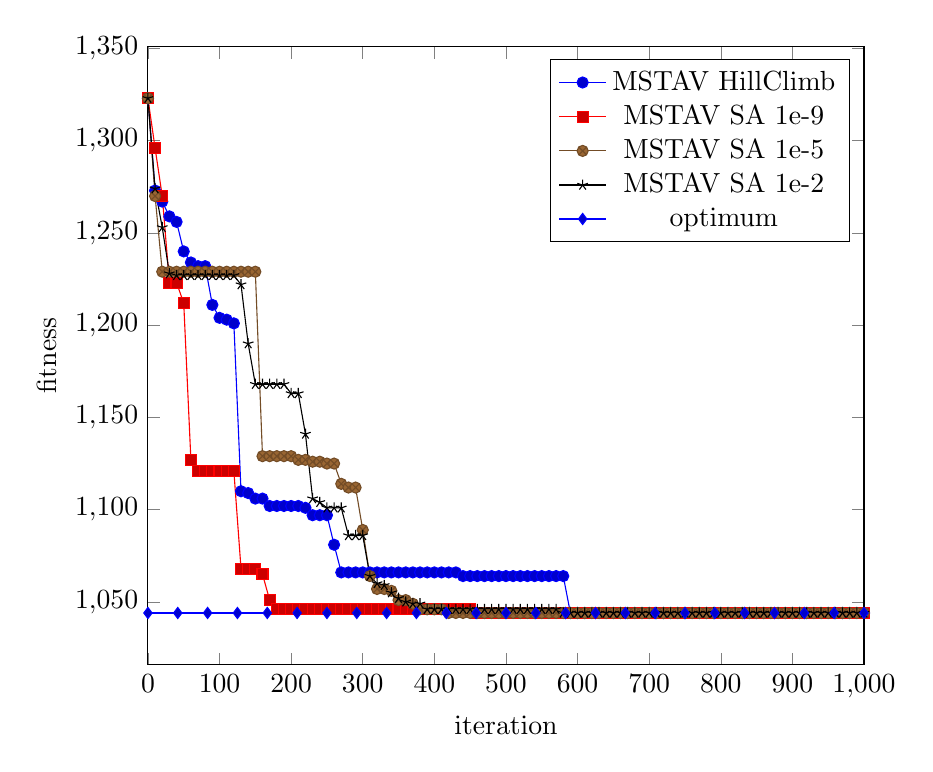
\begin{tikzpicture}
 \begin{axis}[
   width=0.75\textwidth,
   scale only axis,
   xlabel=iteration,
   ylabel=fitness,
   xmin=0,xmax=1000,
   domain=0:1000]
   \addplot coordinates {
     (0,1323)
     (10,1273)
     (20,1267)
     (30,1259)
     (40,1256)
     (50,1240)
     (60,1234)
     (70,1232)
     (80,1232)
     (90,1211)
     (100,1204)
     (110,1203)
     (120,1201)
     (130,1110)
     (140,1109)
     (150,1106)
     (160,1106)
     (170,1102)
     (180,1102)
     (190,1102)
     (200,1102)
     (210,1102)
     (220,1101)
     (230,1097)
     (240,1097)
     (250,1097)
     (260,1081)
     (270,1066)
     (280,1066)
     (290,1066)
     (300,1066)
     (310,1066)
     (320,1066)
     (330,1066)
     (340,1066)
     (350,1066)
     (360,1066)
     (370,1066)
     (380,1066)
     (390,1066)
     (400,1066)
     (410,1066)
     (420,1066)
     (430,1066)
     (440,1064)
     (450,1064)
     (460,1064)
     (470,1064)
     (480,1064)
     (490,1064)
     (500,1064)
     (510,1064)
     (520,1064)
     (530,1064)
     (540,1064)
     (550,1064)
     (560,1064)
     (570,1064)
     (580,1064)
     (590,1044)
     (600,1044)
     (610,1044)
     (620,1044)
     (630,1044)
     (640,1044)
     (650,1044)
     (660,1044)
     (670,1044)
     (680,1044)
     (690,1044)
     (700,1044)
     (710,1044)
     (720,1044)
     (730,1044)
     (740,1044)
     (750,1044)
     (760,1044)
     (770,1044)
     (780,1044)
     (790,1044)
     (800,1044)
     (810,1044)
     (820,1044)
     (830,1044)
     (840,1044)
     (850,1044)
     (860,1044)
     (870,1044)
     (880,1044)
     (890,1044)
     (900,1044)
     (910,1044)
     (920,1044)
     (930,1044)
     (940,1044)
     (950,1044)
     (960,1044)
     (970,1044)
     (980,1044)
     (990,1044)
     (1000,1044)
   };
   \addlegendentry{MSTAV HillClimb}
   \addplot coordinates {
     (0,1323)
     (10,1296)
     (20,1270)
     (30,1223)
     (40,1223)
     (50,1212)
     (60,1127)
     (70,1121)
     (80,1121)
     (90,1121)
     (100,1121)
     (110,1121)
     (120,1121)
     (130,1068)
     (140,1068)
     (150,1068)
     (160,1065)
     (170,1051)
     (180,1046)
     (190,1046)
     (200,1046)
     (210,1046)
     (220,1046)
     (230,1046)
     (240,1046)
     (250,1046)
     (260,1046)
     (270,1046)
     (280,1046)
     (290,1046)
     (300,1046)
     (310,1046)
     (320,1046)
     (330,1046)
     (340,1046)
     (350,1046)
     (360,1046)
     (370,1046)
     (380,1046)
     (390,1046)
     (400,1046)
     (410,1046)
     (420,1046)
     (430,1046)
     (440,1046)
     (450,1046)
     (460,1044)
     (470,1044)
     (480,1044)
     (490,1044)
     (500,1044)
     (510,1044)
     (520,1044)
     (530,1044)
     (540,1044)
     (550,1044)
     (560,1044)
     (570,1044)
     (580,1044)
     (590,1044)
     (600,1044)
     (610,1044)
     (620,1044)
     (630,1044)
     (640,1044)
     (650,1044)
     (660,1044)
     (670,1044)
     (680,1044)
     (690,1044)
     (700,1044)
     (710,1044)
     (720,1044)
     (730,1044)
     (740,1044)
     (750,1044)
     (760,1044)
     (770,1044)
     (780,1044)
     (790,1044)
     (800,1044)
     (810,1044)
     (820,1044)
     (830,1044)
     (840,1044)
     (850,1044)
     (860,1044)
     (870,1044)
     (880,1044)
     (890,1044)
     (900,1044)
     (910,1044)
     (920,1044)
     (930,1044)
     (940,1044)
     (950,1044)
     (960,1044)
     (970,1044)
     (980,1044)
     (990,1044)
     (1000,1044)
   };
   \addlegendentry{MSTAV SA 1e-9}
   \addplot coordinates {
     (0,1323)
     (10,1270)
     (20,1229)
     (30,1229)
     (40,1229)
     (50,1229)
     (60,1229)
     (70,1229)
     (80,1229)
     (90,1229)
     (100,1229)
     (110,1229)
     (120,1229)
     (130,1229)
     (140,1229)
     (150,1229)
     (160,1129)
     (170,1129)
     (180,1129)
     (190,1129)
     (200,1129)
     (210,1127)
     (220,1127)
     (230,1126)
     (240,1126)
     (250,1125)
     (260,1125)
     (270,1114)
     (280,1112)
     (290,1112)
     (300,1089)
     (310,1064)
     (320,1057)
     (330,1057)
     (340,1056)
     (350,1051)
     (360,1051)
     (370,1049)
     (380,1046)
     (390,1046)
     (400,1046)
     (410,1046)
     (420,1044)
     (430,1044)
     (440,1044)
     (450,1044)
     (460,1044)
     (470,1044)
     (480,1044)
     (490,1044)
     (500,1044)
     (510,1044)
     (520,1044)
     (530,1044)
     (540,1044)
     (550,1044)
     (560,1044)
     (570,1044)
     (580,1044)
     (590,1044)
     (600,1044)
     (610,1044)
     (620,1044)
     (630,1044)
     (640,1044)
     (650,1044)
     (660,1044)
     (670,1044)
     (680,1044)
     (690,1044)
     (700,1044)
     (710,1044)
     (720,1044)
     (730,1044)
     (740,1044)
     (750,1044)
     (760,1044)
     (770,1044)
     (780,1044)
     (790,1044)
     (800,1044)
     (810,1044)
     (820,1044)
     (830,1044)
     (840,1044)
     (850,1044)
     (860,1044)
     (870,1044)
     (880,1044)
     (890,1044)
     (900,1044)
     (910,1044)
     (920,1044)
     (930,1044)
     (940,1044)
     (950,1044)
     (960,1044)
     (970,1044)
     (980,1044)
     (990,1044)
     (1000,1044)
   };
   \addlegendentry{MSTAV SA 1e-5}
   \addplot coordinates {
     (0,1323)
     (10,1274)
     (20,1253)
     (30,1228)
     (40,1227)
     (50,1227)
     (60,1227)
     (70,1227)
     (80,1227)
     (90,1227)
     (100,1227)
     (110,1227)
     (120,1227)
     (130,1222)
     (140,1190)
     (150,1168)
     (160,1168)
     (170,1168)
     (180,1168)
     (190,1168)
     (200,1163)
     (210,1163)
     (220,1141)
     (230,1106)
     (240,1104)
     (250,1101)
     (260,1101)
     (270,1101)
     (280,1086)
     (290,1086)
     (300,1086)
     (310,1064)
     (320,1060)
     (330,1059)
     (340,1055)
     (350,1052)
     (360,1050)
     (370,1049)
     (380,1049)
     (390,1046)
     (400,1046)
     (410,1046)
     (420,1046)
     (430,1046)
     (440,1046)
     (450,1046)
     (460,1046)
     (470,1046)
     (480,1046)
     (490,1046)
     (500,1046)
     (510,1046)
     (520,1046)
     (530,1046)
     (540,1046)
     (550,1046)
     (560,1046)
     (570,1046)
     (580,1044)
     (590,1044)
     (600,1044)
     (610,1044)
     (620,1044)
     (630,1044)
     (640,1044)
     (650,1044)
     (660,1044)
     (670,1044)
     (680,1044)
     (690,1044)
     (700,1044)
     (710,1044)
     (720,1044)
     (730,1044)
     (740,1044)
     (750,1044)
     (760,1044)
     (770,1044)
     (780,1044)
     (790,1044)
     (800,1044)
     (810,1044)
     (820,1044)
     (830,1044)
     (840,1044)
     (850,1044)
     (860,1044)
     (870,1044)
     (880,1044)
     (890,1044)
     (900,1044)
     (910,1044)
     (920,1044)
     (930,1044)
     (940,1044)
     (950,1044)
     (960,1044)
     (970,1044)
     (980,1044)
     (990,1044)
     (1000,1044)
   };
   \addlegendentry{MSTAV SA 1e-2}
   \addplot {1044.000000};
   \addlegendentry{optimum}
 \end{axis}
 \end{tikzpicture}
\end{figure}

\pgfsetplotmarksize{0pt}
\begin{figure}
 \centering
 \caption{\label{MSTAV-brasil58}MSTAV-brasil58},
 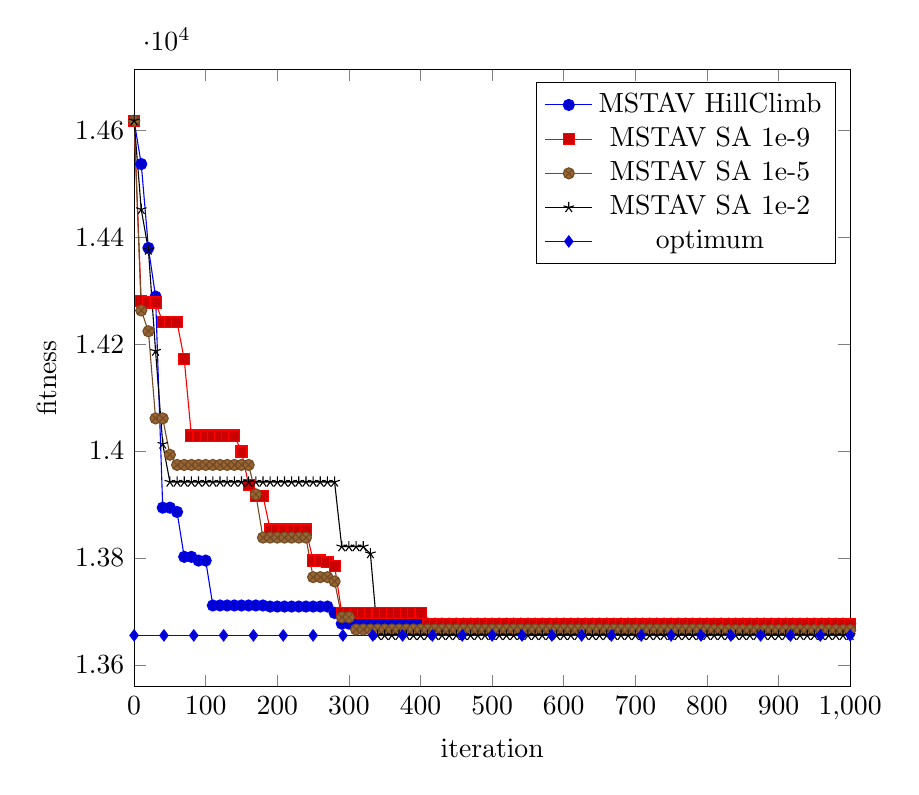
\begin{tikzpicture}
 \begin{axis}[
   width=0.75\textwidth,
   scale only axis,
   xlabel=iteration,
   ylabel=fitness,
   xmin=0,xmax=1000,
   domain=0:1000]
   \addplot coordinates {
     (0,14618)
     (10,14537)
     (20,14380)
     (30,14289)
     (40,13894)
     (50,13894)
     (60,13886)
     (70,13802)
     (80,13802)
     (90,13795)
     (100,13795)
     (110,13711)
     (120,13711)
     (130,13711)
     (140,13711)
     (150,13711)
     (160,13711)
     (170,13711)
     (180,13711)
     (190,13709)
     (200,13709)
     (210,13709)
     (220,13709)
     (230,13709)
     (240,13709)
     (250,13709)
     (260,13709)
     (270,13709)
     (280,13697)
     (290,13677)
     (300,13677)
     (310,13677)
     (320,13677)
     (330,13677)
     (340,13677)
     (350,13677)
     (360,13677)
     (370,13677)
     (380,13677)
     (390,13677)
     (400,13677)
     (410,13677)
     (420,13677)
     (430,13677)
     (440,13677)
     (450,13677)
     (460,13677)
     (470,13677)
     (480,13677)
     (490,13677)
     (500,13677)
     (510,13677)
     (520,13677)
     (530,13677)
     (540,13677)
     (550,13677)
     (560,13677)
     (570,13677)
     (580,13677)
     (590,13677)
     (600,13677)
     (610,13677)
     (620,13677)
     (630,13677)
     (640,13677)
     (650,13677)
     (660,13677)
     (670,13677)
     (680,13677)
     (690,13677)
     (700,13677)
     (710,13677)
     (720,13677)
     (730,13677)
     (740,13677)
     (750,13677)
     (760,13677)
     (770,13677)
     (780,13677)
     (790,13677)
     (800,13677)
     (810,13677)
     (820,13677)
     (830,13677)
     (840,13677)
     (850,13677)
     (860,13677)
     (870,13677)
     (880,13677)
     (890,13677)
     (900,13677)
     (910,13677)
     (920,13677)
     (930,13677)
     (940,13677)
     (950,13677)
     (960,13677)
     (970,13677)
     (980,13677)
     (990,13677)
     (1000,13677)
   };
   \addlegendentry{MSTAV HillClimb}
   \addplot coordinates {
     (0,14618)
     (10,14280)
     (20,14278)
     (30,14278)
     (40,14241)
     (50,14241)
     (60,14241)
     (70,14172)
     (80,14029)
     (90,14029)
     (100,14029)
     (110,14029)
     (120,14029)
     (130,14029)
     (140,14029)
     (150,13999)
     (160,13937)
     (170,13916)
     (180,13916)
     (190,13853)
     (200,13853)
     (210,13853)
     (220,13853)
     (230,13853)
     (240,13853)
     (250,13795)
     (260,13795)
     (270,13793)
     (280,13785)
     (290,13697)
     (300,13697)
     (310,13697)
     (320,13697)
     (330,13697)
     (340,13697)
     (350,13697)
     (360,13697)
     (370,13697)
     (380,13697)
     (390,13697)
     (400,13697)
     (410,13677)
     (420,13677)
     (430,13677)
     (440,13677)
     (450,13677)
     (460,13677)
     (470,13677)
     (480,13677)
     (490,13677)
     (500,13677)
     (510,13677)
     (520,13677)
     (530,13677)
     (540,13677)
     (550,13677)
     (560,13677)
     (570,13677)
     (580,13677)
     (590,13677)
     (600,13677)
     (610,13677)
     (620,13677)
     (630,13677)
     (640,13677)
     (650,13677)
     (660,13677)
     (670,13677)
     (680,13677)
     (690,13677)
     (700,13677)
     (710,13677)
     (720,13677)
     (730,13677)
     (740,13677)
     (750,13677)
     (760,13677)
     (770,13677)
     (780,13677)
     (790,13677)
     (800,13677)
     (810,13677)
     (820,13677)
     (830,13677)
     (840,13677)
     (850,13677)
     (860,13677)
     (870,13677)
     (880,13677)
     (890,13677)
     (900,13677)
     (910,13677)
     (920,13677)
     (930,13677)
     (940,13677)
     (950,13677)
     (960,13677)
     (970,13677)
     (980,13677)
     (990,13677)
     (1000,13677)
   };
   \addlegendentry{MSTAV SA 1e-9}
   \addplot coordinates {
     (0,14618)
     (10,14263)
     (20,14224)
     (30,14061)
     (40,14061)
     (50,13993)
     (60,13974)
     (70,13974)
     (80,13974)
     (90,13974)
     (100,13974)
     (110,13974)
     (120,13974)
     (130,13974)
     (140,13974)
     (150,13974)
     (160,13974)
     (170,13919)
     (180,13838)
     (190,13838)
     (200,13838)
     (210,13838)
     (220,13838)
     (230,13838)
     (240,13838)
     (250,13764)
     (260,13764)
     (270,13764)
     (280,13756)
     (290,13689)
     (300,13689)
     (310,13666)
     (320,13666)
     (330,13666)
     (340,13666)
     (350,13666)
     (360,13666)
     (370,13666)
     (380,13666)
     (390,13666)
     (400,13666)
     (410,13666)
     (420,13666)
     (430,13666)
     (440,13666)
     (450,13666)
     (460,13666)
     (470,13666)
     (480,13666)
     (490,13666)
     (500,13666)
     (510,13666)
     (520,13666)
     (530,13666)
     (540,13666)
     (550,13666)
     (560,13666)
     (570,13666)
     (580,13666)
     (590,13666)
     (600,13666)
     (610,13666)
     (620,13666)
     (630,13666)
     (640,13666)
     (650,13666)
     (660,13666)
     (670,13666)
     (680,13666)
     (690,13666)
     (700,13666)
     (710,13666)
     (720,13666)
     (730,13666)
     (740,13666)
     (750,13666)
     (760,13666)
     (770,13666)
     (780,13666)
     (790,13666)
     (800,13666)
     (810,13665)
     (820,13665)
     (830,13665)
     (840,13665)
     (850,13665)
     (860,13665)
     (870,13665)
     (880,13665)
     (890,13665)
     (900,13665)
     (910,13665)
     (920,13665)
     (930,13665)
     (940,13665)
     (950,13665)
     (960,13665)
     (970,13665)
     (980,13665)
     (990,13665)
     (1000,13665)
   };
   \addlegendentry{MSTAV SA 1e-5}
   \addplot coordinates {
     (0,14618)
     (10,14452)
     (20,14376)
     (30,14187)
     (40,14013)
     (50,13942)
     (60,13942)
     (70,13942)
     (80,13942)
     (90,13942)
     (100,13942)
     (110,13942)
     (120,13942)
     (130,13942)
     (140,13942)
     (150,13942)
     (160,13942)
     (170,13942)
     (180,13942)
     (190,13942)
     (200,13942)
     (210,13942)
     (220,13942)
     (230,13942)
     (240,13942)
     (250,13942)
     (260,13942)
     (270,13942)
     (280,13942)
     (290,13821)
     (300,13821)
     (310,13821)
     (320,13821)
     (330,13808)
     (340,13655)
     (350,13655)
     (360,13655)
     (370,13655)
     (380,13655)
     (390,13655)
     (400,13655)
     (410,13655)
     (420,13655)
     (430,13655)
     (440,13655)
     (450,13655)
     (460,13655)
     (470,13655)
     (480,13655)
     (490,13655)
     (500,13655)
     (510,13655)
     (520,13655)
     (530,13655)
     (540,13655)
     (550,13655)
     (560,13655)
     (570,13655)
     (580,13655)
     (590,13655)
     (600,13655)
     (610,13655)
     (620,13655)
     (630,13655)
     (640,13655)
     (650,13655)
     (660,13655)
     (670,13655)
     (680,13655)
     (690,13655)
     (700,13655)
     (710,13655)
     (720,13655)
     (730,13655)
     (740,13655)
     (750,13655)
     (760,13655)
     (770,13655)
     (780,13655)
     (790,13655)
     (800,13655)
     (810,13655)
     (820,13655)
     (830,13655)
     (840,13655)
     (850,13655)
     (860,13655)
     (870,13655)
     (880,13655)
     (890,13655)
     (900,13655)
     (910,13655)
     (920,13655)
     (930,13655)
     (940,13655)
     (950,13655)
     (960,13655)
     (970,13655)
     (980,13655)
     (990,13655)
     (1000,13655)
   };
   \addlegendentry{MSTAV SA 1e-2}
   \addplot {13655.000000};
   \addlegendentry{optimum}
 \end{axis}
 \end{tikzpicture}
\end{figure}

\pgfsetplotmarksize{0pt}
\begin{figure}
 \centering
 \caption{\label{MSTAV-c10}MSTAV-c10},
 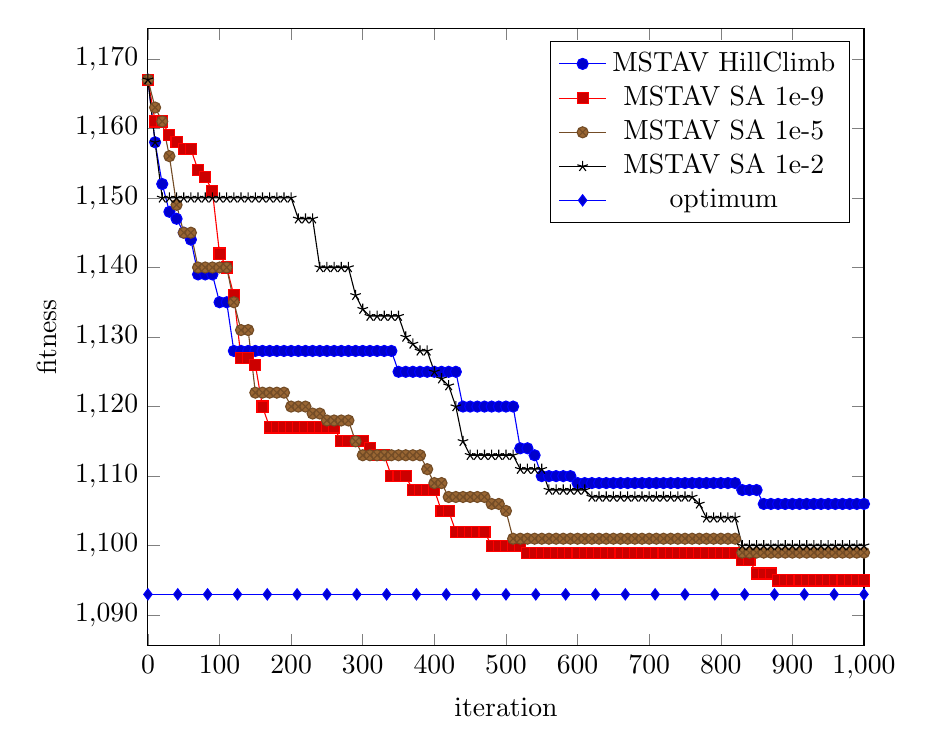
\begin{tikzpicture}
 \begin{axis}[
   width=0.75\textwidth,
   scale only axis,
   xlabel=iteration,
   ylabel=fitness,
   xmin=0,xmax=1000,
   domain=0:1000]
   \addplot coordinates {
     (0,1167)
     (10,1158)
     (20,1152)
     (30,1148)
     (40,1147)
     (50,1145)
     (60,1144)
     (70,1139)
     (80,1139)
     (90,1139)
     (100,1135)
     (110,1135)
     (120,1128)
     (130,1128)
     (140,1128)
     (150,1128)
     (160,1128)
     (170,1128)
     (180,1128)
     (190,1128)
     (200,1128)
     (210,1128)
     (220,1128)
     (230,1128)
     (240,1128)
     (250,1128)
     (260,1128)
     (270,1128)
     (280,1128)
     (290,1128)
     (300,1128)
     (310,1128)
     (320,1128)
     (330,1128)
     (340,1128)
     (350,1125)
     (360,1125)
     (370,1125)
     (380,1125)
     (390,1125)
     (400,1125)
     (410,1125)
     (420,1125)
     (430,1125)
     (440,1120)
     (450,1120)
     (460,1120)
     (470,1120)
     (480,1120)
     (490,1120)
     (500,1120)
     (510,1120)
     (520,1114)
     (530,1114)
     (540,1113)
     (550,1110)
     (560,1110)
     (570,1110)
     (580,1110)
     (590,1110)
     (600,1109)
     (610,1109)
     (620,1109)
     (630,1109)
     (640,1109)
     (650,1109)
     (660,1109)
     (670,1109)
     (680,1109)
     (690,1109)
     (700,1109)
     (710,1109)
     (720,1109)
     (730,1109)
     (740,1109)
     (750,1109)
     (760,1109)
     (770,1109)
     (780,1109)
     (790,1109)
     (800,1109)
     (810,1109)
     (820,1109)
     (830,1108)
     (840,1108)
     (850,1108)
     (860,1106)
     (870,1106)
     (880,1106)
     (890,1106)
     (900,1106)
     (910,1106)
     (920,1106)
     (930,1106)
     (940,1106)
     (950,1106)
     (960,1106)
     (970,1106)
     (980,1106)
     (990,1106)
     (1000,1106)
   };
   \addlegendentry{MSTAV HillClimb}
   \addplot coordinates {
     (0,1167)
     (10,1161)
     (20,1161)
     (30,1159)
     (40,1158)
     (50,1157)
     (60,1157)
     (70,1154)
     (80,1153)
     (90,1151)
     (100,1142)
     (110,1140)
     (120,1136)
     (130,1127)
     (140,1127)
     (150,1126)
     (160,1120)
     (170,1117)
     (180,1117)
     (190,1117)
     (200,1117)
     (210,1117)
     (220,1117)
     (230,1117)
     (240,1117)
     (250,1117)
     (260,1117)
     (270,1115)
     (280,1115)
     (290,1115)
     (300,1115)
     (310,1114)
     (320,1113)
     (330,1113)
     (340,1110)
     (350,1110)
     (360,1110)
     (370,1108)
     (380,1108)
     (390,1108)
     (400,1108)
     (410,1105)
     (420,1105)
     (430,1102)
     (440,1102)
     (450,1102)
     (460,1102)
     (470,1102)
     (480,1100)
     (490,1100)
     (500,1100)
     (510,1100)
     (520,1100)
     (530,1099)
     (540,1099)
     (550,1099)
     (560,1099)
     (570,1099)
     (580,1099)
     (590,1099)
     (600,1099)
     (610,1099)
     (620,1099)
     (630,1099)
     (640,1099)
     (650,1099)
     (660,1099)
     (670,1099)
     (680,1099)
     (690,1099)
     (700,1099)
     (710,1099)
     (720,1099)
     (730,1099)
     (740,1099)
     (750,1099)
     (760,1099)
     (770,1099)
     (780,1099)
     (790,1099)
     (800,1099)
     (810,1099)
     (820,1099)
     (830,1098)
     (840,1098)
     (850,1096)
     (860,1096)
     (870,1096)
     (880,1095)
     (890,1095)
     (900,1095)
     (910,1095)
     (920,1095)
     (930,1095)
     (940,1095)
     (950,1095)
     (960,1095)
     (970,1095)
     (980,1095)
     (990,1095)
     (1000,1095)
   };
   \addlegendentry{MSTAV SA 1e-9}
   \addplot coordinates {
     (0,1167)
     (10,1163)
     (20,1161)
     (30,1156)
     (40,1149)
     (50,1145)
     (60,1145)
     (70,1140)
     (80,1140)
     (90,1140)
     (100,1140)
     (110,1140)
     (120,1135)
     (130,1131)
     (140,1131)
     (150,1122)
     (160,1122)
     (170,1122)
     (180,1122)
     (190,1122)
     (200,1120)
     (210,1120)
     (220,1120)
     (230,1119)
     (240,1119)
     (250,1118)
     (260,1118)
     (270,1118)
     (280,1118)
     (290,1115)
     (300,1113)
     (310,1113)
     (320,1113)
     (330,1113)
     (340,1113)
     (350,1113)
     (360,1113)
     (370,1113)
     (380,1113)
     (390,1111)
     (400,1109)
     (410,1109)
     (420,1107)
     (430,1107)
     (440,1107)
     (450,1107)
     (460,1107)
     (470,1107)
     (480,1106)
     (490,1106)
     (500,1105)
     (510,1101)
     (520,1101)
     (530,1101)
     (540,1101)
     (550,1101)
     (560,1101)
     (570,1101)
     (580,1101)
     (590,1101)
     (600,1101)
     (610,1101)
     (620,1101)
     (630,1101)
     (640,1101)
     (650,1101)
     (660,1101)
     (670,1101)
     (680,1101)
     (690,1101)
     (700,1101)
     (710,1101)
     (720,1101)
     (730,1101)
     (740,1101)
     (750,1101)
     (760,1101)
     (770,1101)
     (780,1101)
     (790,1101)
     (800,1101)
     (810,1101)
     (820,1101)
     (830,1099)
     (840,1099)
     (850,1099)
     (860,1099)
     (870,1099)
     (880,1099)
     (890,1099)
     (900,1099)
     (910,1099)
     (920,1099)
     (930,1099)
     (940,1099)
     (950,1099)
     (960,1099)
     (970,1099)
     (980,1099)
     (990,1099)
     (1000,1099)
   };
   \addlegendentry{MSTAV SA 1e-5}
   \addplot coordinates {
     (0,1167)
     (10,1158)
     (20,1150)
     (30,1150)
     (40,1150)
     (50,1150)
     (60,1150)
     (70,1150)
     (80,1150)
     (90,1150)
     (100,1150)
     (110,1150)
     (120,1150)
     (130,1150)
     (140,1150)
     (150,1150)
     (160,1150)
     (170,1150)
     (180,1150)
     (190,1150)
     (200,1150)
     (210,1147)
     (220,1147)
     (230,1147)
     (240,1140)
     (250,1140)
     (260,1140)
     (270,1140)
     (280,1140)
     (290,1136)
     (300,1134)
     (310,1133)
     (320,1133)
     (330,1133)
     (340,1133)
     (350,1133)
     (360,1130)
     (370,1129)
     (380,1128)
     (390,1128)
     (400,1125)
     (410,1124)
     (420,1123)
     (430,1120)
     (440,1115)
     (450,1113)
     (460,1113)
     (470,1113)
     (480,1113)
     (490,1113)
     (500,1113)
     (510,1113)
     (520,1111)
     (530,1111)
     (540,1111)
     (550,1111)
     (560,1108)
     (570,1108)
     (580,1108)
     (590,1108)
     (600,1108)
     (610,1108)
     (620,1107)
     (630,1107)
     (640,1107)
     (650,1107)
     (660,1107)
     (670,1107)
     (680,1107)
     (690,1107)
     (700,1107)
     (710,1107)
     (720,1107)
     (730,1107)
     (740,1107)
     (750,1107)
     (760,1107)
     (770,1106)
     (780,1104)
     (790,1104)
     (800,1104)
     (810,1104)
     (820,1104)
     (830,1100)
     (840,1100)
     (850,1100)
     (860,1100)
     (870,1100)
     (880,1100)
     (890,1100)
     (900,1100)
     (910,1100)
     (920,1100)
     (930,1100)
     (940,1100)
     (950,1100)
     (960,1100)
     (970,1100)
     (980,1100)
     (990,1100)
     (1000,1100)
   };
   \addlegendentry{MSTAV SA 1e-2}
   \addplot {1093.000000};
   \addlegendentry{optimum}
 \end{axis}
 \end{tikzpicture}
\end{figure}


\subsection{CBC and MSTAV convergence comparison}
STUB text\\
TODO: napisac, ze MSTAV > CRC, zasugerowac dlaczego\\
TODO: dodac CBC SA do analizy
\pgfsetplotmarksize{0pt}
 \centering
 \caption{\label{CBCvsMSTAV-01sEV100K30}CBCvsMSTAV-01sEV100K30},
 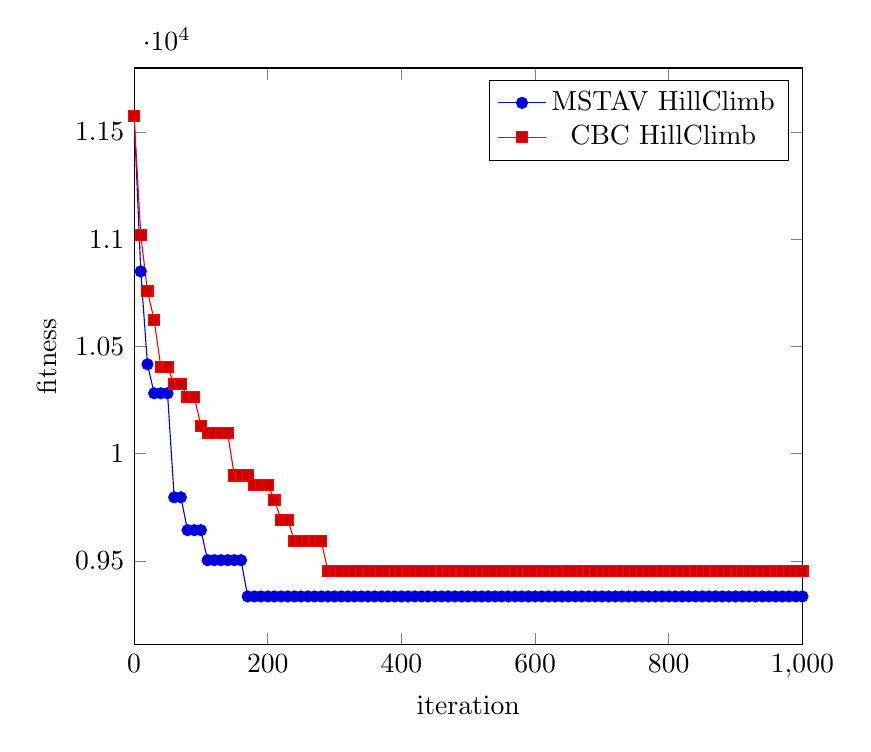
\begin{tikzpicture}
 \begin{axis}[
   width=0.7\textwidth,
   scale only axis,
   xlabel=iteration,
   ylabel=fitness,
   xmin=0,xmax=1000,
   domain=0:1000]
   \addplot coordinates {
     (0,11574)
     (10,10850)
     (20,10417)
     (30,10282)
     (40,10282)
     (50,10282)
     (60,9797)
     (70,9797)
     (80,9644)
     (90,9644)
     (100,9644)
     (110,9504)
     (120,9504)
     (130,9504)
     (140,9504)
     (150,9504)
     (160,9504)
     (170,9335)
     (180,9335)
     (190,9335)
     (200,9335)
     (210,9335)
     (220,9335)
     (230,9335)
     (240,9335)
     (250,9335)
     (260,9335)
     (270,9335)
     (280,9335)
     (290,9335)
     (300,9335)
     (310,9335)
     (320,9335)
     (330,9335)
     (340,9335)
     (350,9335)
     (360,9335)
     (370,9335)
     (380,9335)
     (390,9335)
     (400,9335)
     (410,9335)
     (420,9335)
     (430,9335)
     (440,9335)
     (450,9335)
     (460,9335)
     (470,9335)
     (480,9335)
     (490,9335)
     (500,9335)
     (510,9335)
     (520,9335)
     (530,9335)
     (540,9335)
     (550,9335)
     (560,9335)
     (570,9335)
     (580,9335)
     (590,9335)
     (600,9335)
     (610,9335)
     (620,9335)
     (630,9335)
     (640,9335)
     (650,9335)
     (660,9335)
     (670,9335)
     (680,9335)
     (690,9335)
     (700,9335)
     (710,9335)
     (720,9335)
     (730,9335)
     (740,9335)
     (750,9335)
     (760,9335)
     (770,9335)
     (780,9335)
     (790,9335)
     (800,9335)
     (810,9335)
     (820,9335)
     (830,9335)
     (840,9335)
     (850,9335)
     (860,9335)
     (870,9335)
     (880,9335)
     (890,9335)
     (900,9335)
     (910,9335)
     (920,9335)
     (930,9335)
     (940,9335)
     (950,9335)
     (960,9335)
     (970,9335)
     (980,9335)
     (990,9335)
     (1000,9335)
   };
   \addlegendentry{MSTAV HillClimb}
   \addplot coordinates {
     (0,11574)
     (10,11020)
     (20,10758)
     (30,10624)
     (40,10405)
     (50,10405)
     (60,10324)
     (70,10324)
     (80,10265)
     (90,10265)
     (100,10130)
     (110,10095)
     (120,10095)
     (130,10095)
     (140,10095)
     (150,9899)
     (160,9899)
     (170,9899)
     (180,9856)
     (190,9856)
     (200,9856)
     (210,9786)
     (220,9690)
     (230,9690)
     (240,9595)
     (250,9595)
     (260,9595)
     (270,9595)
     (280,9595)
     (290,9454)
     (300,9454)
     (310,9454)
     (320,9454)
     (330,9454)
     (340,9454)
     (350,9454)
     (360,9454)
     (370,9454)
     (380,9454)
     (390,9454)
     (400,9454)
     (410,9454)
     (420,9454)
     (430,9454)
     (440,9454)
     (450,9454)
     (460,9454)
     (470,9454)
     (480,9454)
     (490,9454)
     (500,9454)
     (510,9454)
     (520,9454)
     (530,9454)
     (540,9454)
     (550,9454)
     (560,9454)
     (570,9454)
     (580,9454)
     (590,9454)
     (600,9454)
     (610,9454)
     (620,9454)
     (630,9454)
     (640,9454)
     (650,9454)
     (660,9454)
     (670,9454)
     (680,9454)
     (690,9454)
     (700,9454)
     (710,9454)
     (720,9454)
     (730,9454)
     (740,9454)
     (750,9454)
     (760,9454)
     (770,9454)
     (780,9454)
     (790,9454)
     (800,9454)
     (810,9454)
     (820,9454)
     (830,9454)
     (840,9454)
     (850,9454)
     (860,9454)
     (870,9454)
     (880,9454)
     (890,9454)
     (900,9454)
     (910,9454)
     (920,9454)
     (930,9454)
     (940,9454)
     (950,9454)
     (960,9454)
     (970,9454)
     (980,9454)
     (990,9454)
     (1000,9454)
   };
   \addlegendentry{CBC HillClimb}
 \end{axis}
 \end{tikzpicture}

\pgfsetplotmarksize{0pt}
 \centering
 \caption{\label{CBCvsMSTAV-01sRV1000K150}CBCvsMSTAV-01sRV1000K150},
 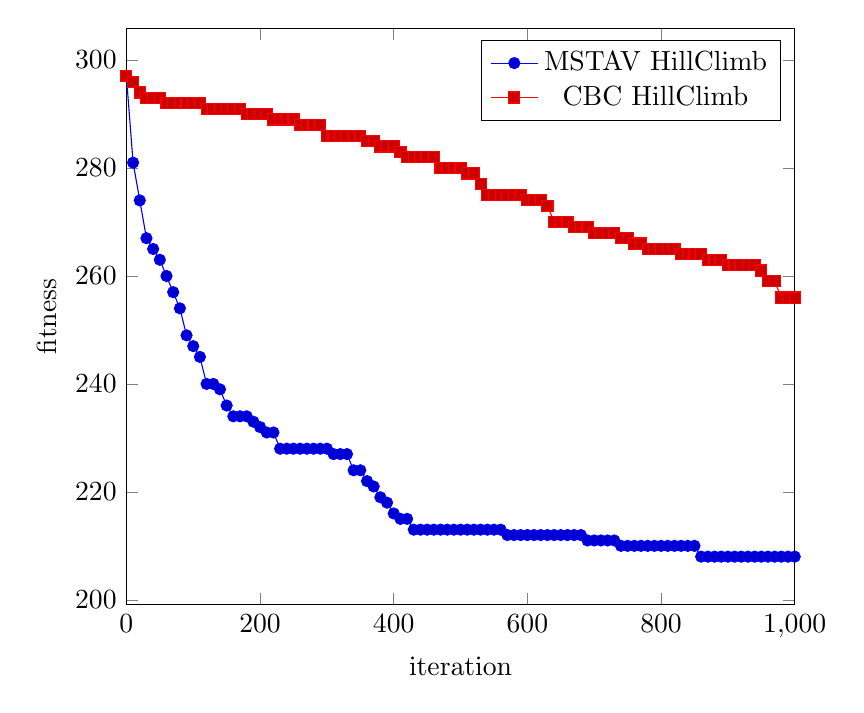
\begin{tikzpicture}
 \begin{axis}[
   width=0.7\textwidth,
   scale only axis,
   xlabel=iteration,
   ylabel=fitness,
   xmin=0,xmax=1000,
   domain=0:1000]
   \addplot coordinates {
     (0,297)
     (10,281)
     (20,274)
     (30,267)
     (40,265)
     (50,263)
     (60,260)
     (70,257)
     (80,254)
     (90,249)
     (100,247)
     (110,245)
     (120,240)
     (130,240)
     (140,239)
     (150,236)
     (160,234)
     (170,234)
     (180,234)
     (190,233)
     (200,232)
     (210,231)
     (220,231)
     (230,228)
     (240,228)
     (250,228)
     (260,228)
     (270,228)
     (280,228)
     (290,228)
     (300,228)
     (310,227)
     (320,227)
     (330,227)
     (340,224)
     (350,224)
     (360,222)
     (370,221)
     (380,219)
     (390,218)
     (400,216)
     (410,215)
     (420,215)
     (430,213)
     (440,213)
     (450,213)
     (460,213)
     (470,213)
     (480,213)
     (490,213)
     (500,213)
     (510,213)
     (520,213)
     (530,213)
     (540,213)
     (550,213)
     (560,213)
     (570,212)
     (580,212)
     (590,212)
     (600,212)
     (610,212)
     (620,212)
     (630,212)
     (640,212)
     (650,212)
     (660,212)
     (670,212)
     (680,212)
     (690,211)
     (700,211)
     (710,211)
     (720,211)
     (730,211)
     (740,210)
     (750,210)
     (760,210)
     (770,210)
     (780,210)
     (790,210)
     (800,210)
     (810,210)
     (820,210)
     (830,210)
     (840,210)
     (850,210)
     (860,208)
     (870,208)
     (880,208)
     (890,208)
     (900,208)
     (910,208)
     (920,208)
     (930,208)
     (940,208)
     (950,208)
     (960,208)
     (970,208)
     (980,208)
     (990,208)
     (1000,208)
   };
   \addlegendentry{MSTAV HillClimb}
   \addplot coordinates {
     (0,297)
     (10,296)
     (20,294)
     (30,293)
     (40,293)
     (50,293)
     (60,292)
     (70,292)
     (80,292)
     (90,292)
     (100,292)
     (110,292)
     (120,291)
     (130,291)
     (140,291)
     (150,291)
     (160,291)
     (170,291)
     (180,290)
     (190,290)
     (200,290)
     (210,290)
     (220,289)
     (230,289)
     (240,289)
     (250,289)
     (260,288)
     (270,288)
     (280,288)
     (290,288)
     (300,286)
     (310,286)
     (320,286)
     (330,286)
     (340,286)
     (350,286)
     (360,285)
     (370,285)
     (380,284)
     (390,284)
     (400,284)
     (410,283)
     (420,282)
     (430,282)
     (440,282)
     (450,282)
     (460,282)
     (470,280)
     (480,280)
     (490,280)
     (500,280)
     (510,279)
     (520,279)
     (530,277)
     (540,275)
     (550,275)
     (560,275)
     (570,275)
     (580,275)
     (590,275)
     (600,274)
     (610,274)
     (620,274)
     (630,273)
     (640,270)
     (650,270)
     (660,270)
     (670,269)
     (680,269)
     (690,269)
     (700,268)
     (710,268)
     (720,268)
     (730,268)
     (740,267)
     (750,267)
     (760,266)
     (770,266)
     (780,265)
     (790,265)
     (800,265)
     (810,265)
     (820,265)
     (830,264)
     (840,264)
     (850,264)
     (860,264)
     (870,263)
     (880,263)
     (890,263)
     (900,262)
     (910,262)
     (920,262)
     (930,262)
     (940,262)
     (950,261)
     (960,259)
     (970,259)
     (980,256)
     (990,256)
     (1000,256)
   };
   \addlegendentry{CBC HillClimb}
 \end{axis}
 \end{tikzpicture}

\pgfsetplotmarksize{0pt}
 \centering
 \caption{\label{CBCvsMSTAV-d05}CBCvsMSTAV-d05},
 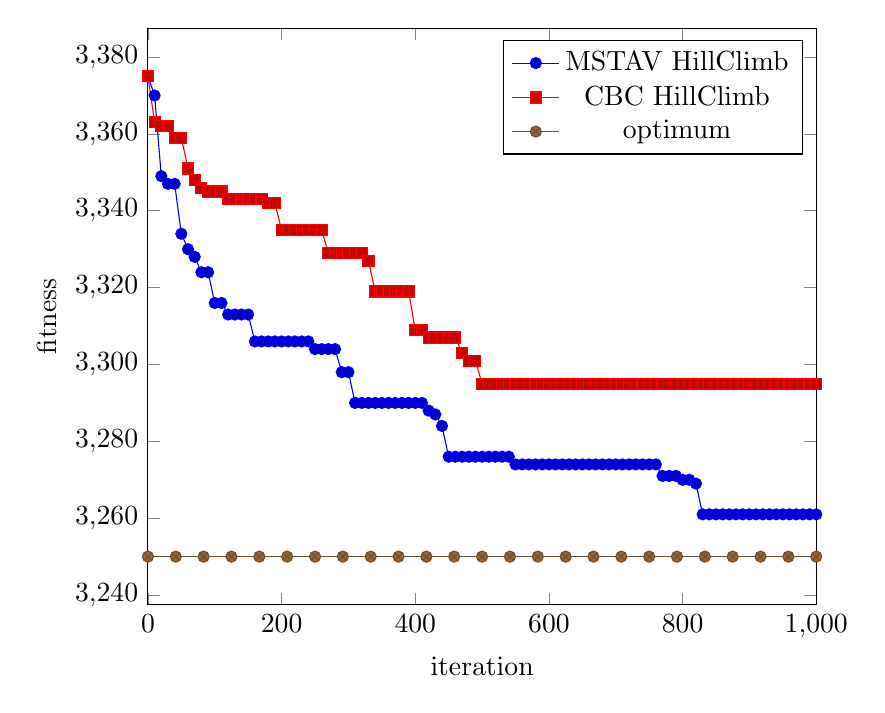
\begin{tikzpicture}
 \begin{axis}[
   width=0.7\textwidth,
   scale only axis,
   xlabel=iteration,
   ylabel=fitness,
   xmin=0,xmax=1000,
   domain=0:1000]
   \addplot coordinates {
     (0,3375)
     (10,3370)
     (20,3349)
     (30,3347)
     (40,3347)
     (50,3334)
     (60,3330)
     (70,3328)
     (80,3324)
     (90,3324)
     (100,3316)
     (110,3316)
     (120,3313)
     (130,3313)
     (140,3313)
     (150,3313)
     (160,3306)
     (170,3306)
     (180,3306)
     (190,3306)
     (200,3306)
     (210,3306)
     (220,3306)
     (230,3306)
     (240,3306)
     (250,3304)
     (260,3304)
     (270,3304)
     (280,3304)
     (290,3298)
     (300,3298)
     (310,3290)
     (320,3290)
     (330,3290)
     (340,3290)
     (350,3290)
     (360,3290)
     (370,3290)
     (380,3290)
     (390,3290)
     (400,3290)
     (410,3290)
     (420,3288)
     (430,3287)
     (440,3284)
     (450,3276)
     (460,3276)
     (470,3276)
     (480,3276)
     (490,3276)
     (500,3276)
     (510,3276)
     (520,3276)
     (530,3276)
     (540,3276)
     (550,3274)
     (560,3274)
     (570,3274)
     (580,3274)
     (590,3274)
     (600,3274)
     (610,3274)
     (620,3274)
     (630,3274)
     (640,3274)
     (650,3274)
     (660,3274)
     (670,3274)
     (680,3274)
     (690,3274)
     (700,3274)
     (710,3274)
     (720,3274)
     (730,3274)
     (740,3274)
     (750,3274)
     (760,3274)
     (770,3271)
     (780,3271)
     (790,3271)
     (800,3270)
     (810,3270)
     (820,3269)
     (830,3261)
     (840,3261)
     (850,3261)
     (860,3261)
     (870,3261)
     (880,3261)
     (890,3261)
     (900,3261)
     (910,3261)
     (920,3261)
     (930,3261)
     (940,3261)
     (950,3261)
     (960,3261)
     (970,3261)
     (980,3261)
     (990,3261)
     (1000,3261)
   };
   \addlegendentry{MSTAV HillClimb}
   \addplot coordinates {
     (0,3375)
     (10,3363)
     (20,3362)
     (30,3362)
     (40,3359)
     (50,3359)
     (60,3351)
     (70,3348)
     (80,3346)
     (90,3345)
     (100,3345)
     (110,3345)
     (120,3343)
     (130,3343)
     (140,3343)
     (150,3343)
     (160,3343)
     (170,3343)
     (180,3342)
     (190,3342)
     (200,3335)
     (210,3335)
     (220,3335)
     (230,3335)
     (240,3335)
     (250,3335)
     (260,3335)
     (270,3329)
     (280,3329)
     (290,3329)
     (300,3329)
     (310,3329)
     (320,3329)
     (330,3327)
     (340,3319)
     (350,3319)
     (360,3319)
     (370,3319)
     (380,3319)
     (390,3319)
     (400,3309)
     (410,3309)
     (420,3307)
     (430,3307)
     (440,3307)
     (450,3307)
     (460,3307)
     (470,3303)
     (480,3301)
     (490,3301)
     (500,3295)
     (510,3295)
     (520,3295)
     (530,3295)
     (540,3295)
     (550,3295)
     (560,3295)
     (570,3295)
     (580,3295)
     (590,3295)
     (600,3295)
     (610,3295)
     (620,3295)
     (630,3295)
     (640,3295)
     (650,3295)
     (660,3295)
     (670,3295)
     (680,3295)
     (690,3295)
     (700,3295)
     (710,3295)
     (720,3295)
     (730,3295)
     (740,3295)
     (750,3295)
     (760,3295)
     (770,3295)
     (780,3295)
     (790,3295)
     (800,3295)
     (810,3295)
     (820,3295)
     (830,3295)
     (840,3295)
     (850,3295)
     (860,3295)
     (870,3295)
     (880,3295)
     (890,3295)
     (900,3295)
     (910,3295)
     (920,3295)
     (930,3295)
     (940,3295)
     (950,3295)
     (960,3295)
     (970,3295)
     (980,3295)
     (990,3295)
     (1000,3295)
   };
   \addlegendentry{CBC HillClimb}
   \addplot {3250.000000};
   \addlegendentry{optimum}
 \end{axis}
 \end{tikzpicture}

\pgfsetplotmarksize{0pt}
\begin{figure}
 \centering
 \caption{\label{CBCvsMSTAV-gap1307}CBCvsMSTAV-gap1307},
 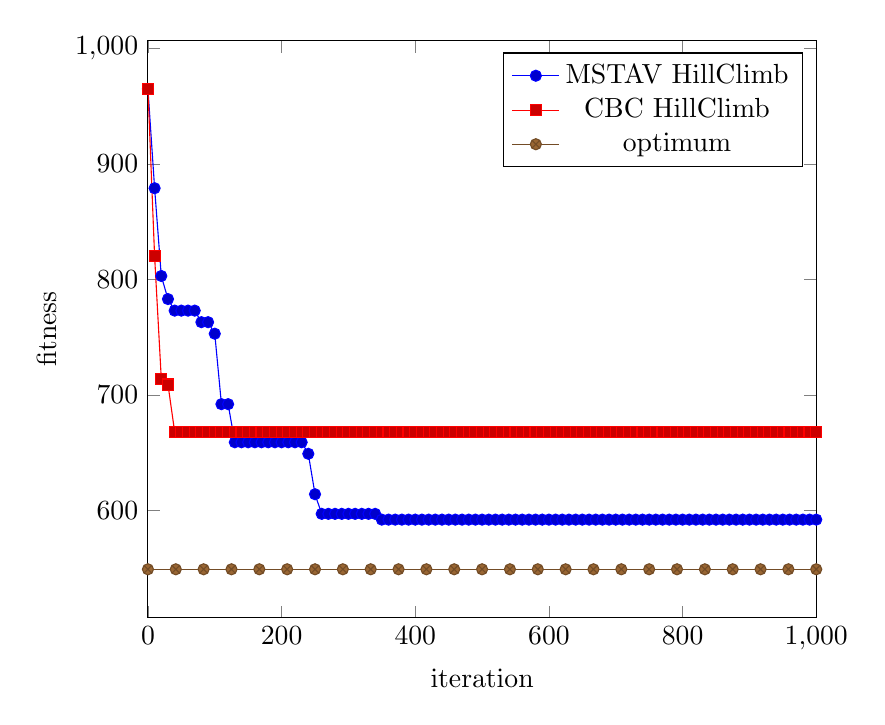
\begin{tikzpicture}
 \begin{axis}[
   width=0.7\textwidth,
   scale only axis,
   xlabel=iteration,
   ylabel=fitness,
   xmin=0,xmax=1000,
   domain=0:1000]
   \addplot coordinates {
     (0,965)
     (10,879)
     (20,803)
     (30,783)
     (40,773)
     (50,773)
     (60,773)
     (70,773)
     (80,763)
     (90,763)
     (100,753)
     (110,692)
     (120,692)
     (130,659)
     (140,659)
     (150,659)
     (160,659)
     (170,659)
     (180,659)
     (190,659)
     (200,659)
     (210,659)
     (220,659)
     (230,659)
     (240,649)
     (250,614)
     (260,597)
     (270,597)
     (280,597)
     (290,597)
     (300,597)
     (310,597)
     (320,597)
     (330,597)
     (340,597)
     (350,592)
     (360,592)
     (370,592)
     (380,592)
     (390,592)
     (400,592)
     (410,592)
     (420,592)
     (430,592)
     (440,592)
     (450,592)
     (460,592)
     (470,592)
     (480,592)
     (490,592)
     (500,592)
     (510,592)
     (520,592)
     (530,592)
     (540,592)
     (550,592)
     (560,592)
     (570,592)
     (580,592)
     (590,592)
     (600,592)
     (610,592)
     (620,592)
     (630,592)
     (640,592)
     (650,592)
     (660,592)
     (670,592)
     (680,592)
     (690,592)
     (700,592)
     (710,592)
     (720,592)
     (730,592)
     (740,592)
     (750,592)
     (760,592)
     (770,592)
     (780,592)
     (790,592)
     (800,592)
     (810,592)
     (820,592)
     (830,592)
     (840,592)
     (850,592)
     (860,592)
     (870,592)
     (880,592)
     (890,592)
     (900,592)
     (910,592)
     (920,592)
     (930,592)
     (940,592)
     (950,592)
     (960,592)
     (970,592)
     (980,592)
     (990,592)
     (1000,592)
   };
   \addlegendentry{MSTAV HillClimb}
   \addplot coordinates {
     (0,965)
     (10,820)
     (20,714)
     (30,709)
     (40,668)
     (50,668)
     (60,668)
     (70,668)
     (80,668)
     (90,668)
     (100,668)
     (110,668)
     (120,668)
     (130,668)
     (140,668)
     (150,668)
     (160,668)
     (170,668)
     (180,668)
     (190,668)
     (200,668)
     (210,668)
     (220,668)
     (230,668)
     (240,668)
     (250,668)
     (260,668)
     (270,668)
     (280,668)
     (290,668)
     (300,668)
     (310,668)
     (320,668)
     (330,668)
     (340,668)
     (350,668)
     (360,668)
     (370,668)
     (380,668)
     (390,668)
     (400,668)
     (410,668)
     (420,668)
     (430,668)
     (440,668)
     (450,668)
     (460,668)
     (470,668)
     (480,668)
     (490,668)
     (500,668)
     (510,668)
     (520,668)
     (530,668)
     (540,668)
     (550,668)
     (560,668)
     (570,668)
     (580,668)
     (590,668)
     (600,668)
     (610,668)
     (620,668)
     (630,668)
     (640,668)
     (650,668)
     (660,668)
     (670,668)
     (680,668)
     (690,668)
     (700,668)
     (710,668)
     (720,668)
     (730,668)
     (740,668)
     (750,668)
     (760,668)
     (770,668)
     (780,668)
     (790,668)
     (800,668)
     (810,668)
     (820,668)
     (830,668)
     (840,668)
     (850,668)
     (860,668)
     (870,668)
     (880,668)
     (890,668)
     (900,668)
     (910,668)
     (920,668)
     (930,668)
     (940,668)
     (950,668)
     (960,668)
     (970,668)
     (980,668)
     (990,668)
     (1000,668)
   };
   \addlegendentry{CBC HillClimb}
   \addplot {549.000000};
   \addlegendentry{optimum}
 \end{axis}
 \end{tikzpicture}
\end{figure}


\subsection{Comparison of found solutions' cost}
STUB text
TODO: napisac, ze na malych testach, praktycznie zawsze MSTAV jest bliski lub lepszy od apx,
na srednich testach bywa roznie, ale zazwyczaj wciaz MSTAV daje rade,
na duzych roznica jest zdecydowana
TODO: na malych testach CBC radzi sobie dosc dobrze
TODO: dodac CBC SA do analizy
\begin{figure}[ht]
  \centering
  \begin{tabular}[ht]{|l||c|c|c|c|H}
\cline{1-5}
 & 01dEV100K20 & 01sEV100K20 & 01dRV100K20 & 01sRV100K30 & \\ \cline{1-5}\cline{1-5} 
2-Approximation &3476 & 5927 & 24 & 105 & \\ \cline{1-5}
MSTAV HillClimb &3403 & 5785 & 22 & 94 & \\ \cline{1-5}
CBC HillClimb &3496 & 6021 & 24 & 101 & \\ \cline{1-5}
\end{tabular}
\end{figure}

\begin{figure}[ht]
  \centering
  \begin{tabular}[ht]{|l||c|c|c|c|c|c|H}
\cline{1-7}
 & alut2764 & b13 & berlin52 & diw0250 & msm3277 & d15 & \\ \cline{1-7}\cline{1-7} 
Optimum &640 & 165 & 1044 & 350 & 869 & 1116 & \\ \cline{1-7}
2-Approximation &710 & 187 & 1078 & 363 & 912 & 1161 & \\ \cline{1-7}
MSTAV HillClimb &662 & 170 & 1044 & 467 & 1089 & 1126 & \\ \cline{1-7}
CBC HillClimb &1044 & 177 & 1103 & 518 & 1222 & 1186 & \\ \cline{1-7}
\end{tabular}
\end{figure}

\begin{figure}[ht]
  \centering
  \begin{tabular}[ht]{|l||c|c|c|c|H}
\cline{1-5}
 & 04sEV1000K250 & 03sEV1000K150 & 01sRV1000K150 & 01sRV1000K250 & \\ \cline{1-5}\cline{1-5} 
2-Approximation &29569 & 17175 & 208 & 262 & \\ \cline{1-5}
MSTAV HillClimb &29624 & 17163 & 196 & 279 & \\ \cline{1-5}
CBC HillClimb &35091 & 21899 & 259 & 365 & \\ \cline{1-5}
\end{tabular}
\end{figure}

\begin{figure}[ht]
  \centering
  \begin{tabular}[ht]{|l||c|c|c|c|c|c|H}
\cline{1-7}
 & alue2087 & d11 & diw0445 & e02 & taq0431 & msm3277 & \\ \cline{1-7}\cline{1-7} 
Optimum &1049 & 29 & 1363 & 214 & 897 & 869 & \\ \cline{1-7}
2-Approximation &1122 & 33 & 1453 & 255 & 980 & 912 & \\ \cline{1-7}
MSTAV HillClimb &1375 & 36 & 1827 & 361 & 1484 & 1233 & \\ \cline{1-7}
CBC HillClimb &1698 & 49 & 2321 & 442 & 1519 & 1263 & \\ \cline{1-7}
\end{tabular}
\end{figure}

